\documentclass[reprint,aps,prb]{revtex4-1}

% Language and font encodings
\usepackage[english]{babel}

% Useful packages
\usepackage{graphicx}
\usepackage{subfig}
\usepackage{amsmath,amsfonts,amssymb,amsthm}
\usepackage{mathtools,braket}
\usepackage{tikz}
\usepackage{xifthen}
%\pgfplotsset{compat=1.15}

% notation for standard math
\renewcommand{\d}{\partial}
\newcommand{\half}{\frac{1}{2}}
\newcommand{\dd}{{\rm d}}
\renewcommand{\r}{{\bf r}}
\newcommand{\br}{\bar{\bf r}}
\newcommand{\x}{{\bf x}}
\newcommand{\eps}{\epsilon}
\newcommand{\bomega}{\bar\omega}
\newcommand{\bbomega}{\bar{\bomega}}
\newcommand{\ii}{\mathrm{i}}
\newcommand{\intdef}[3]{\int_{#1}^{#2} \dd {#3}}
\newcommand{\intover}[1]{\int_{-\infty}^{+\infty} \dd {#1}}
\newcommand{\sint}{\mathrlap{\displaystyle\int}
\mathrlap{\textstyle\sum}
\phantom{\mathrlap{\displaystyle
\int}\textstyle\sum}}

% notatiotion for equation environments
\newcommand{\be}{\begin{equation}}
\newcommand{\ee}{\end{equation}}
\newcommand{\ba}{\begin{eqnarray}}
\newcommand{\ea}{\end{eqnarray}}
\newcommand{\baa}{\begin{align}}
\newcommand{\eaa}{\end{align}}
\newcommand{\nn}{\notag}
\newcommand{\qq}{\qquad}
\newcommand{\lb}{\label}
\newcommand{\mat}[1]{\begin{pmatrix} #1\end{pmatrix}}

% notation for the operators
\newcommand{\op}[1]{\hat {#1}}
\newcommand{\sop}[1]{\op{\op {#1}}}
\newcommand{\commutator}[2]{\left[ {#1} , {#2} \right]}
\newcommand{\trace}[1]{\mathrm{tr}\left(#1\right)}
\newcommand{\argument}[1]{\ifthenelse{\isempty{#1}{}}{}{(#1)}}
\newcommand{\matop}[1]{\mathbf{#1}}
\newcommand{\optr}[1]{\check #1}
\newcommand{\opskew}[1]{{\op {#1}}_{\perp}}

% notation for the states
\newcommand{\tket}[1]{| \tilde #1 \rangle}
\newcommand{\tbra}[1]{\langle \tilde #1 |}
\newcommand{\brket}[2]{\langle  #1 | #2 \rangle} %standard braket
\newcommand{\tbraket}[2]{\langle \tilde #1 | #2 \rangle}
\newcommand{\ketbra}[2]{| #1 \rangle \langle #2 |}
\newcommand{\tketbra}[2]{| #1 \rangle \langle \tilde #2 |}
\newcommand{\sket}[2]{| #2)^{#1}}
\newcommand{\sbra}[2]{( #2|_{#1}}
\newcommand{\sketor}[2]{| #2]^{#1}}
\newcommand{\sbraor}[2]{[ #2|_{#1}}
\newcommand{\sbraket}[2]{\braket{\op{#1} | \op{#2}}}
\newcommand{\dket}[1]{\Bigl| #1 \Bigr)}
\newcommand{\dbra}[1]{\Bigl(#1 \Bigr|}
\newcommand{\dbraket}[2]{\Bigl(#1 \Bigl| #2 \Bigr)}
\newcommand{\dketor}[1]{\Bigl| #1 \Bigr]}
\newcommand{\dbraor}[1]{\Bigl[#1 \Bigr|}
\newcommand{\hket}[1]{| #1 ]}
\newcommand{\hbra}[1]{[ #1 |}
\newcommand{\hbraket}[2]{[#1 | #2 ]}

% special operators
\newcommand{\dmnot}{\op{\rho}_0}
\newcommand{\dm}{\op{\rho}}
\newcommand{\hnot}{\op{H}_0}
\newcommand{\hone}[1]{\op{H}_1\argument{#1}}
\newcommand{\transition}[1]{\op T_{#1}}
\newcommand{\excite}[2]{\op e_{{#1}{#2}}}
\newcommand{\decay}[2]{\op d_{{#1}{#2}}}
\newcommand{\Liouv}{\sop{\mathcal L}}
\newcommand{\Liouvnot}{\sop{\mathcal L_0}}
\newcommand{\coupl}{\sop{\mathcal K}}
\newcommand{\honetmp}[1][]{\op{H_1}\argument{#1}} 
\newcommand{\identity}{\op{\mathbb I}}
\newcommand{\rmat}[1]{\optr R}
\newcommand{\fscd}[1]{\ket{f_p^\Phi(\omega)^{#1}}}

\captionsetup{justification=centerlast}

\begin{document}

%\preprint{APS/123-QED}

%\title{On the analytic structure of the linear response susceptibility in open systems}
\title{Locality and Computational Reliability of Linear Response Calculations for Molecular Systems}% Localization properties, observable character and computational reliability of the linear response in open systems}
\author{Marco D'Alessandro}%
\affiliation{Istituto di Struttura della Materia-CNR (ISM-CNR), Via del Fosso del Cavaliere 100, 00133 Roma, Italia}
\author{Luigi Genovese}
\affiliation{Laboratoire de Simulation Atomistique (LSim), SP2M, INAC, CEA-UJF, 17 Av. des Martyrs,
38054 Grenoble, France}
\date{\today}

\begin{abstract}
By performing a critical analysis of the fundamental equations of linear-response  (LR) formalisms in molecules, 
we explore the interplay between locality of the response density operator and  numerical convergence of LR-related quantities.
We show that the first ionization potential of the system behaves as a threshold energy: for frequencies below this value, it is possible to parametrize the response density by employing localized states only. Above this threshold, such a locality property cannot be achieved. 
Such considerations may be transposed in terms of the molecule's excited states. We show that not all the system's excitations can be considered on equal footing.
There is a discrete sector of excitations that can be parametrized by observable, localized states, which can be computationally expressed with high precision, provided an adequate level of completeness. 
We present indicators that can help to quantify such potential observable property of an excitation, that can be evaluated 
in any discretization scheme.  
The remaining excitation modes belong to a continuum spectrum that, on the contrary, is not directly associated to observable properties and can only be effectively represented in a given computational setup.
Such considerations are important not only for reproducibility of the results among different computer codes 
employing diverse formalisms, but also in view of providing a deeper understanding on the impact of models' 
approximations on the scientific outcomes of the simulation.

% ---
% We discuss these aspects in the context of linear response treatment of molecular systems. 
% By analysing simple case-studies with a highly complete numerical formalism, 
% we explore the interplay between locality of the perturbed wavefunctions and 
% numerical convergence of observable quantities. This will enable us to draw some considerations on the analytic structure of the linear susceptivity for open systems and on the potential convergence issues that might arise in a given computational setup.

% We believe that such discussion could provide useful considerations and perspectives for the design of a effective approaches for the study of molecular excitations in realistic conditions.

% We analyze how the fundamental equations which govern the linear response properties of a quantum system are influenced by the presence of open boundaries.
% In particular we focus our attention on linear-response (LR)-TDDFT calculation of molecular systems.
% Above this energy threshold, the excitation spectrum may be separated in two sectors: one can still be described in terms of observable excitation 
% with discrete energies, that can be captured within computational setups tailored for localized states. 
% This result is a inherent behavior of the system's Liouvillian, and does not depend on computational treatment of the 
% unoccupied subspace.
\end{abstract}

%\pacs{Valid PACS appear here}
\maketitle

\section{Introduction}
Since the days of their foundations, disciplines like Computational Physics or Quantum Chemistry always had to deal with the problem of the 
computational reliability of the results. More specifically, a computational result may be considered as reliable for various reasons.
It might be, for example, in agreement with some previous observation or measurement that the employed computational model is susceptible to reproduce.
The model itself may in this way be classified as ``accurate''; it can then be employed to extract, \textit{in silico},
other quantities that might be then used to \emph{predict} or \emph{interpret} experiments.
Another concept of reliability is the concept of  ``precision'', which is more focused to the actual results
that a given computational model provides for a specific set of quantities, regardless of their potential agreement with 
experimental data. The aim of precise computational approach is to reduce the \emph{computational} uncertainties
of quantities extracted out of a well-defined model, and provide reference results, to which other computer codes
employing the same model can be compared.

A recent, remarkable example of precision-driven initiative is provided by the DeltaCodes project~\cite{deltaTest2016},
where a grassroot community of code-owners struggled to extract well-defined computational results in the context of 
Density Functional Theory (DFT) calculations. Ground-State quantum mechanical quantities as lattice constants and bulk modulus of 
elementary crystals extracted from different codes were compared with each other, with the objective of reducing the uncertainties 
on such data, and in some sense, to define a \emph{calibration} procedure for a Solid-State Physics DFT code. 
Any other code able to extract the same quantities with the same approximations may be compared with the 
results of the community in order to assess its computational reliability.

For a theoretical approach that is based on numerical calculations, for which no analytic reference solution exists, 
reducing the computational uncertainty is the only possible way to shed light on the predictivity power of the
model. In other terms, the ``accuracy'' of a result with respect to experimental data may be reliably quantified
only when the computational uncertainty is guaranteed to be significantly lower than the found discrepancy.
For communities like DFT, such a ``calibration'' of computer codes among each other is a discipline that is still in its infancy;
the DeltaCodes initiative and the foundations of DFT are separated in time by more than 50 years, and the computational
model employed in the comparison (the Perdew-Burke-Erzerhof functional~\cite{PBE}) has been introduced more than 20 years ago.

The problem is even more stringent for calculations that refer to quantities \emph{beyond} ground state, like
for instance the time-dependent density functional theory (TDDFT) \cite{casida1995,runge1984,onida2002},
from which quantities like optical excitations or polarizability tensors
of a given system might be studied and put in relation with experimental data.
Here also, a plethora of computational approaches exist, that employ different numerical formalism and
basis sets, and it will be of great importance to identify quantities that can be ``measured'' in a given model, to assess
and quantify their computational uncertainty.

In this paper, we focus our attention to Linear-Response treatments of \emph{molecular} systems, 
in particular referring to LR-TDDFT calculation. We will investigate the impact that 
\emph{open} (i.e. Isolated) Boundary Conditions (BC) that have to be imposed to the system will have on the computational evaluation of LR quantities.
In order to do this, we perform analytic considerations on the equations beyond LR treatment.
Such considerations will enable us to distinguish quantities that \textit{a priori} can be compared among different treatments - and therefore tested for reproducibility - 
from others that would \emph{explicitly} depend of the the employed computational treatment. 
In particular, we will discuss the interplay between reproducible LR quantities and the \emph{locality} of the related objects.
% In order to do this, we perform analytic considerations on the equations beyond LR treatment,
% which will help us identifying how to distinguish -- \textit{a priori} -- quantities that are susceptible to be 
% compared among different treatments, as they are \emph{intrinsically} associated to localized objects,
% from quantities that \emph{explicitly} depend of the the employed computational treatment.

The paper is organized as follows.
Initially we will inspect how the question of reproducibility may be expressed 
for ground state calculations of molecules. 
Following these guidelines, we will then move to LR equations,
by first considering the equations of motion of the response density operator, given
the application of a perturbing field.
Then we will consider the behaviour of the ``free oscillations'', i.e. the excited states
of the molecule.
Our considerations will also reveal useful for the understanding of the \emph{analytic structure} of LR quantities like
the linear susceptibility of the system (i.e. the reducible polarizability).
We support our considerations with numerical results on simple LR-TDDFT quantities.
For readability purposes, the details of each calculation are explained in the appendix.

Although we refer, as anticipated, to TDDFT models, such considerations might also be transposed to Many-Body Perturbation Theory
approaches, in the context Quasi-Particle equations.

% Moreover, wheareas for Ground-State calculations the quantities are relatively easy to identify and extract,
% TD-DFT and more generally, linear-response calculation present a further difficulty, which is the problem
% of \emph{numerical} convergence. In other terms, beyond ground state, 
% the absence of tools like the variational theorem imposes us to focus on \emph{well-defined} quantites,
% and to study the conditions under which numerical convergence of the results can be achieved.



% The subject of the present investigation concerns with the study of isolated molecular-like systems subjected to a time-dependent perturbation. % in the linear response regime.
% This problem can be tackled within the contest of the time-dependent density functional theory (TD-DFT) \cite{runge1984,onida2002}, that allows one to establish the time-dependent 
% Kohn-Sham (KS) equations which determine the evolution of the one-particle properties of the system with respect to time. 
% 
% We focus our attention to the linear response regime (LR) in which the theory can be conveniently expressed in the frequency domain and the time-dependent KS equation are reformulated 
% as a quantum Liouville equation for the response density operator. Different computational approaches have been developed in literature \cite{baroni2008,hubener2014,brabec2015}, principally 
% with the aim of producing efficient algorithms for the evaluation of the physical observables. These methods differ both for the procedure adopted to solve the Liouville equation 
% (explicit diagonalization, self-consistent Sternheimer equation, Lanczos chain-like procedure, etc.) and both for the choice of the basis set employed to perform the calculations. 
% Nonetheless, in all the cases one is a dealing with a finite basis set that, unavoidably, gives rise to a limited computational domain. 
% It is then meaningful to try to understand under 
% which extent the computational-induced truncation of the natural open boundaries condition could produce observable effects on the physical quantities computed in the LR. 
% 
% A preliminary understanding of this problem can be achieved thanks to the results reported in \cite{boffi2016}. The authors of this paper discuss the effects of a finite basis set on the 
% occupied and virtual orbitals of a molecular system and establish a clear correspondence between the orbital localization character, and the independence of its properties (\emph{e.g.} energy) 
% with respect to the basis set. It is shown that (localized) orbitals with a bound-state behavior in the long range constitute a genuine discrete set and a finite basis is 
% able to provide a reliable description of these states if the sampled domain contains their natural sizes. On the contrary, unbound (delocalized) orbitals form a continuum of states in the 
% true system with open boundaries. For these class of objects the presence of a finite computational domain has a deeper impact since introduces a fictitious discretization of the energy levels. 
% Furthermore, the energies of the unbound orbitals are not stable with respect to a change of the size of the computational domain and approach to zero as long as it is increased.  
% 
% In this paper we aim to reach a deeper understanding of the possible effects of a finite computational basis set on the LR regime in open systems. To achieve this task we try to
% reformulate the relation between localization properties and basis independence for the main actors of the LR formalism. We present a discussion based on a double level analysis. First, 
% we propose a localization argument directly based on the inspection of the response density operator. Then, we move to a deeper level and investigate the properties of the susceptibility 
% functional, which represents the fundamental object in the contest of the linear response. Pursuing this approach we are naturally led to investigate the localization properties of excitation 
% operators, that in turn emerge as the resonant channel of the spectral decomposition of the susceptibility. In this way we establish a direct relation between the concept of basis independence 
% and the analytic structure of the linear response susceptibility.

% First of all it is useful to discuss the property of the ground state under this perspective. 
% Indeed, it is well known that the stability of the ground state and the localized nature of a molecular-like system ensures that the KS description of occupied states is represented 
% by a discrete set of wave functions that approaches to zero far apart from a compact region around the system's atoms. This behavior indicates that a (finite) basis set will provide 
% a reliable description of the ground state properties if it is able to sample a computational domain which contains the natural sizes of the occupied orbitals \cite{boffi2016}.
% The same arguments cannot be rigidly extended to the case in which an external time-dependent field starts acting on the system. Indeed, the perturbation drives the system out 
% from the equilibrium and the electrons sample a wider region of the state space, that will contains orbitals of both negative (bound) and positive (unbound) energies. 

%\section{Localization properties of the linear response actors in open systems}
\subsection{Long range behavior of the eigenvalue solution of the Schr\"odinger equation}
\label{SEopenSystem}

Let us start our discussion by revisiting the impact that the Isolated BC have on the 
solutions of the time-independent Schr\"odinger Equation.
We here present well-known concepts of elementary quantum mechanics, under a perspective that
will turn out to be very useful in the forthcoming considerations about linear-response quantities.

Consider a (one-body) wavefunction $\ket{\psi}$ solution of the equation
$\op H\ket{\psi}=\eps\ket{\psi}$, where we split the Hamiltonian operator into the sum of
a kinetic $\op T$ and a potential $\op V \equiv \op H - \op T$ term.
In view of analysing the impact of the BC, it is instructive to transform 
the Schr\"odinger equation in a scattering problem, by writing
\be\lb{SEHelmholtz1}
\ket{\psi} = \op G_H(\eps)\ket{\op V\psi}\;,
\ee
where we have introduced the Green function of the Helmholtz operator $\op G_H(\eps) = (\eps-\op T)^{-1}$,
resolvent of the free-particle Hamiltonian $H_s \equiv \op T$.

When describing the Ground State of a molecule, we suppose that the potential operator, even if non-local,
can be effectively restricted on wavefunctions that can be considered as nonzero only on a
bounded domain. In other terms, a molecule can be associated to a ``scatterer'' that has a \emph{finite} 
spatial extension; if a state $\ket{\psi}$ is localized, it will be the same for the ket $\ket{\op V \psi}$, though 
perhaps in a larger region.
For a computational analysis of the problem, this property is fundamental in the choice of the numerical treatment as we know that
computational basis sets 
that are tailored to express asymptotically vanishing wavefunctions are better suited for the solution of the problem.

This fact is made apparent by the expression of 
the kernel of $\op G_H(\eps)$ in the coordinate representation. 
When dealing with Isolated BC, it is easy to see that the solution of Eq.~\eqref{SEHelmholtz1}
can be expressed by:
\be\lb{HelmholtzKernelDef1}
\bra{\r} \op G_H(\eps) \ket{\r'} = \frac{1}{4\pi} \begin{cases}
\frac{e^{-\alpha|\r - \r' |}}{|\r- \r' |} \;,\; & {\textrm for}\; \eps  < 0\; \\ 
\frac{e^{\ii \alpha |\r-\r' |}}{|\r-\r' |} \;, & {\textrm for} \; \eps \geq 0
\end{cases} \;,
\ee
where $\alpha = \sqrt{2|\eps|}$. 

From the above expressions we can see that, for molecular systems,the value $\epsilon=0$
represents a \emph{threshold}~\footnote{The threshold value in general should correspond to asymptotic value of the potential at infinity.} 
energy that separates two different classes of solutions.
Negative-energy solutions are \emph{localized}, i.e. they exhibit bound-state behavior far away from the scatterer.
These are bound states and, by means of their normalizability, they are associated to \emph{discrete}, well-defined energies.
The bound states can be of course labelled by quantum numbers that are defined by the properties of the scatterer, namely the
symmetries of the potential $\op V$.
In a computational discretization of the Schr\"odinger equation, such states can be in principle expressed with arbitrary precision, 
provided that the numerical treatment offers the adequate level of completeness. 
Being discrete and well-identified, the bound-state energies are a property of the molecule and can be associated to \emph{observable}
quantities. The values of their energies can be compared among different treatments and it is in principle possible to
provide reference results on them.


On the other hand, positive energy solutions behave differently. 
Even though the potential is localized, their positive energy makes them behave 
as spherical waves and its convolution with the source term  gives raise to a delocalized wavefunction $\psi(\r)$ 
in the whole accessible space.
As they cannot be normalized they belong to the essential spectrum of the Hamiltonian operator and form a \emph{continuum} of states.
Thanks to the Lippmann-Schwinger relation of Eq.~\eqref{SEHelmholtz1} they can be put in bijection with the eigenstates of the 
free-particle Hamiltonian $\op H_s$. We may say that their quantum numbers are determined by the Laplacian operator, 
regardless of the particular features of the potential.

It is easy to see from these concepts that a computational treatment that is tailored for the discretization of bound states
will not be effective for continuum states, due to the different long-range asymptotic behavior - which in turn is a clear consequence of the 
BC of the problem. In a numerical treatment, discretizing the problem with a \emph{finite}
number of degrees of freedom, we will only have access to a \emph{pseudo}-continuum of states,
whose energy values and density of states will depend on the representation of the kinetic operator
in the basis set. As a consequence, numerical eigenstates with $\epsilon > 0$ will have a value of their energy that will \emph{always}
depend on the computational setup.

A direct numerical evidence of this problem has been discussed in \cite{boffi2016}. The authors of this paper analyze the effects of a finite basis set on the 
occupied and virtual orbitals of a molecular system and establish a clear correspondence between the orbital localization character, 
and the independence of its energy with respect to the basis set. 
% It is shown that (localized) orbitals with a bound-state behavior in the long range constitute a genuine discrete set and a finite basis is 
% able to provide a reliable description of these states if the sampled domain contains their natural sizes. On the contrary, unbound (delocalized) orbitals form a continuum of states in the 
% true system with open boundaries. For these class of objects the presence of a finite computational domain has a deeper impact since introduces a fictitious discretization of the energy levels. 
On the contrary, it is clearly shown that the energies of the unbound orbitals are not stable with respect to a change of the size of the computational domain and approach to zero as long as it is increased.  


\section{Fluctuation states. A localization argument for the response density}
It is evident that the arguments presented in the above section have a limited interest for the study
of Ground State quantities of molecules. By definition, all these quantities can be expressed as a 
functional which \emph{entirely} depends on bound states. As an illustration it is sufficient to recall
the Hohenberg-Kohn theorem that states that the Ground-State (GS) energy is a functional of the GS
charge density $\dmnot$. For molecular systems that are electronically stable (i.e. no anionic or metastable configurations),
such quantity is localized, in the sense of the above section. Stated otherwise, 
\emph{there is no need to express efficiently any portion of the continuum spectrum} to have a reliable GS treatment of molecules.

Let us now inspect the case of LR calculations.
%Linear response can be effectively applied to the analysis of the electronic excitations in open systems.
In this framework one consider the unperturbed Hamiltonian $\hnot$ and assume that 
the GS density $\dmnot$ is accessible and expressed in a given computational treatment. 
The linear response formalism allows us to evaluate the modification of the expectation value of a generic observable induced by a 
time (or frequency)-dependent perturbing field $\op\Phi(\omega)$ acting on the system. 
This quantity, written in the frequency domain, can be expressed through the evaluation of the \emph{linear response functional}
\be\lb{LinearResponseFunctDef1}
\braket{\delta\op O}_\Phi(\omega) = \trace{\dm'_\Phi(\omega)\op O} \;,
\ee
where $\op O$ represents the observable\footnote{For a sake of concreteness, we are limiting our considerations to observables that do not explicitly depend on time} under inspection 
and we have introduced the \emph{response density operator} $\dm'_\Phi(\omega)$ that codifies the modification of $\dmnot$ induced by the perturbation $\op\Phi(\omega)$. 

%The main objective of this section is to investigate the structure of the building blocks needed to express the response density operator. In particular, we are interested in clarifying 
%the behavior of the main actors of the LR in the long range, \emph{i.e.} outside from the support domain of the potential. 




% As a preliminary step for the forthcoming discussion we present a simple argument that allows us to determine the asymptotic character of the eigenvalue solution of the Schr\"odinger equation (SE) 
% $\op H\ket{\psi}=\eps\ket{\psi}$. The main aims of this analysis, apart from reproducing the well known behavior of the wave functions, is to introduce some tools and setting up notations and 
% terminology that will we widely used in the rest of the paper. 
% 
% The argument proceeds by splitting the Hamiltonian as the sum of the kinetic $\op T$ and potential $\op V$ term. Since we are dealing with molecular-like systems $\op V$ has a compact support when 
% projected in the $\r$-representation. We can formally solve the SE as an inhomogeneous Helmholtz equation by writing
% \be\lb{SEHelmholtz1}
% \ket{\psi} = \op G_H(\eps)\ket{\op V\psi}\;,
% \ee
% where we have introduced the Green function of the Helmholtz operator $\op G_H(\eps) = (\eps-\op T)^{-1}$. We observe that, due to the properties of $\op V$, the \emph{source term} $\ket{\op V\psi}$ 
% of equation \eqref{SEHelmholtz1} is localized in space and, for open boundary conditions in three dimensions, the kernel of $\op G_H(\eps)$ in the coordinate representation reads: 
% \be\lb{HelmholtzKernelDef1}
% \bra{\r} \op G_H(\eps) \ket{\r'} = \frac{1}{4\pi} \begin{cases}
% \frac{e^{-\alpha|\r - \r' |}}{|\r- \r' |} \;,\; & {\textrm for}\; \eps  < 0\; \\ 
% \frac{e^{\ii \alpha |\r-\r' |}}{|\r-\r' |} \;, & {\textrm for} \; \eps \geq 0
% \end{cases} \;,
% \ee
% where $\alpha = \sqrt{2|\eps|}$. 
% This representation of the eigenvalues solution of the SE evidences that the value $\eps=0$ represents the threshold level that determines the asymptotic character of the wave functions. 
% Indeed, for $\eps > 0$,  $\op G_H(\eps)$ behaves as a spherical wave and its convolution with the source term  gives raise to a $\psi(\r)$ delocalized in the whole accessible space. Instead, 
% for values of $\eps < 0$, the kernel contains an exponential damping factor and the associated wave functions exhibit a bound-state behavior in the long range. Finally, we observe that the 
% square-integrability and the continuity of the wave function and its derivatives poses further constrains responsible for the discretization of the energy spectrum for bound-states.  
% 
% The different asymptotic behavior of the wave functions has a deep impact on the possible computational induced error obtained when this quantities are evaluated using a (finite) computational
% setup. 



\label{FluctuationState}

The response density operator is expressed as the first-order variation of $\dmnot=\sum_{\{p\}} \ket{\psi_p} \bra{\psi_p}$, where the set $\{\ket{\psi_p}\}$ denote the 
occupied states, \emph{i.e} the subset of the bound eigenstates\footnote{In what follows we will assume that the set of states $\{\ket{\psi_p}\}$ are described by real 
functions, when projected in the $\r$-representation.} of $\hnot$ with (negative) energy $\eps_p$ lower than the Fermi level. Using this notation we denote the energy of the HOMO level 
as $\eps_h$ and identify the value of the first ionization potential with IP~$\equiv|\eps_h|$. 

The response density satisfies an equation of motion written in the form of a quantum Liouville operator (for example see \cite{baroni2008})
\be\lb{LiouvillianRhopomegaDef1}
\left(\omega - \Liouv\right) \dm'_\Phi(\omega) =  \commutator{\op\Phi(\omega)}{\dmnot} \;,
\ee
where $\op\Phi(\omega)$ represents the perturbing field. 
The Liouvillian superoperator $\Liouv$ for self-consistent systems is expressed as the sum of the unperturbed part plus a coupling term. The action of these 
terms reads, respectively
\be\lb{LiouZeroDef1}
\Liouv \op O \equiv \left(\Liouvnot + \coupl \right) \op O = \commutator{\hnot}{\op O} +\commutator{\op V'[\op O]}{\dmnot}  \;,
\ee
where $\op V'[\op O] \equiv \int \dd \r \dd \r'\frac{\delta \op V[\dmnot]}{\delta \rho(\r,\r')} O(\r,\r')$.

The inspection of the linear order time evolution of the eigenstates of $\hnot$ evidence that the response density acts as a transition 
operator, linking the occupied and empty subspaces of $\hnot$, and satisfies the \emph{transverse} condition  
\be\lb{RhopTransverseDef1}
\dm'_\Phi = \dm_{\perp} \doteq \dmnot\dm'_\Phi\op Q_0 + \op Q_0\dm'_\Phi\dmnot \;,
\ee
where $\op Q_0=\identity-\dmnot$ is the projector in the subspace orthogonal to the occupied states of $\hnot$. 
Due to this fact we can introduce an explicit representation of the 
response density parametrized as
\be\lb{rhoPrimeFluctuationStateDef1}
\dm'_\Phi(\omega) = \sum_p\left(\ketbra{\psi_p}{f_p^\Phi(-\omega)} + \ketbra{f_p^\Phi(\omega)}{\psi_p}\right) \;.
\ee
Here we have introduced the set of $\omega$-dependent \emph{fluctuation states} 
$\ket{f_p^\Phi(\omega)} = \dm'_\Phi(\omega) \ket{\psi_p}$, that have values in the unoccupied subspace of $\hnot$. 
An analysis of the Liouville equation \eqref{LiouvillianRhopomegaDef1} for the response density written in this fashion evidences that the equations of motion of fluctuation states are 
written as a modified Sternheimer equation~\cite{mahan1980,giustino2012,giustino2014}
\be\lb{fluctuationStateEqMotion1}
\left[\omega - (\hnot-\eps_p)\right]\ket{f_p^\Phi(\omega)} = \op Q_0(\op\Phi(\omega)+\op V'[\dm'_\Phi](\omega))\ket{\psi_p} \;,
\ee
and we observe that the first-order Hamiltonian contains, 
apart from the perturbing field, a further term $\op V'[\dm'_\Phi]$ due to the density-dependence of $\hnot$.
% The interesting aspect of these equations in the perspective of the present analysis is that they allow us to present a localization argument for the fluctuation states using a procedure  
% analogous to the one depicted in section \ref{SEopenSystem}. So we split the unperturbed Hamiltonian as the sum of the kinetic $\op T$ and potential $\op V$ term and express the solution of 
% \eqref{fluctuationStateEqMotion1} in the form of a self-consistent inhomogeneous Helmholtz equation
It is easy to see that the solution of equation \eqref{fluctuationStateEqMotion1} can be casted in the form of
a set of scattering problems:
%a self-consistent inhomogeneous Helmholtz equation
\be\lb{rhoPrimeFluctuationStateDef2}
\ket{f_p^\Phi(\omega)} = \op G_H(\omega+\epsilon_p)\left(\op V\ket{f_p^\Phi(\omega)} + \ket{s_p^\Phi(\omega)} \right)\;,
\ee
with%:here in this case the source term contains further addend apart from the unperturbed potential and reads:
$%\be
\ket{s_p^\Phi(\omega)} = \op Q_0(\op V'[\dm'_\Phi](\omega) + \op \Phi(\omega))\ket{\psi_p}
$. %\ee

It can be seen that for each choice of $p$, the value $\omega = |\eps_p|$ represents the threshold level 
that govern the localization properties of the corresponding fluctuation state.
As a \emph{stringent} hypothesis, let us now assume that the ket $\ket{s_p^\Phi(\omega)}$ is localized, namely its evaluation can be
restricted on a bounded real-space domain.
%The localization character of fluctuation states can be assessed by following the same argument discussed in section \ref{SEopenSystem} for the eigenstates of the SE. In this case 
%the source term depends also from the perturbation added to the system so this analysis applies only to the class 
%of perturbing field for which $\ket{\op\Phi\psi_p}$ is localized, when projected
%in the $\r$-representation. 
Even when such locality argument holds true, for $\omega > |\eps_p|$, 
the Helmholtz kernel behaves as a spherical wave and  gives raise to a $\ket{f^\Phi_p(\omega)}$ which is \emph{delocalized} in the entire real-space domain.
Such delocalization is an intrinsic consequence of the value of $\omega$, and does not depend on the particular choice of 
$\op \Phi$.
Only for $\omega < |\eps_p|$ the kernel contains an exponential damping factor and $\ket{f^\Phi_p(\omega)}$ exhibits a bound-state behavior in the long range, 
once again provided that the above locality arguments on $\ket{s_p^\Phi(\omega)}$ -- hence on $\op V'$ and $\Phi$ -- are valid.

Such locality property of the fluctuation state can be directly confirmed for static perturbations at $\omega=0$.
Let us consider a static perturbing operator $\op\Phi_s$ that can be restricted to a finite domain. 
Any local operator, like \emph{e.g.} a static electric field $\mathbf F$, with associated scalar potential $\Phi_s[\mathbf F](\r) = -\mathbf F \cdot \r$, would satisfy such property.
We consider the perturbed hamiltonian $\hnot[\dm_{\Phi_s}] + \op\Phi_s[\mathbf F]$, where $\dm_{\Phi_s}$ represents the GS density of the perturbed system, and assume that the 
perturbation strength ($|\mathbf F|$ in the above example) is sufficiently small to be consistent with a LR treatment of the problem. 
In this case, the occupied eigenfunction $\ket{\psi_p^{\Phi_s}}$ of the perturbed hamiltonian can be extracted with traditional GS techniques, 
as from the discussion around Eq.~\eqref{SEHelmholtz1}, they exhibit bound-state behavior.\footnote{The fulfilling of Eq.~\eqref{SEHelmholtz1} for energies below threshold
is not \textit{per se} a guarantee of a localized $\ket{\psi}$. With such equation we demonstrate that, \emph{in the case when} a localized
solution exists, this cannot be found for energies above threshold.}
\begin{figure}[t]
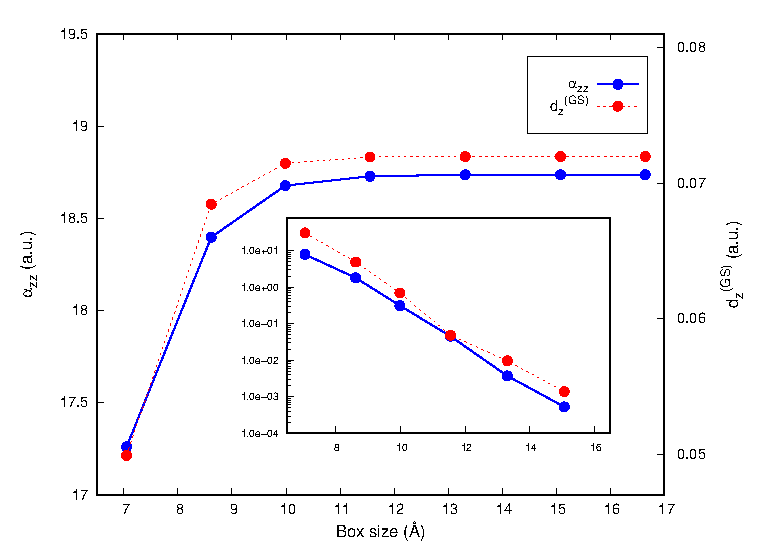
\includegraphics[scale=0.68]{CO_statPolvsBox.eps}
\caption{\label{co_alphaStatic}(Color online) Convergence of the statical polarizability (blue continuous line) and of the ground state permanent dipole (red dotted line) 
of the $CO$ molecule with respect to the size of the computational domain. The inset plot evidences the relative percentage convergence using the value associated to the largest 
box as reference.}
\end{figure}

From the linearized Schr\"odinger Equation of the perturbed problem, it is easy to see that the fluctuation state at $\omega=0$ can be expressed
in terms of the corresponding bound state of the perturbed Hamiltonian, i.e.
$\ket{f_p^{\Phi_s}(0)} \simeq \op Q_0 \ket{\psi_p^{\Phi_s}}$.
For any value of $p$, the locality of the $\ket{f_p^{\Phi_s}(0)}$ therefore directly stems from the
bound-state behavior of $\ket{\psi_p^{\Phi_s}}$. As $\omega=0$ is by hypothesis 
lower than any of the $|\eps_p|$, this is consistent with the above considerations.

Such observations enable us to express quantities like the static polarizability tensor $\alpha_{ij}$ from GS calculations of the perturbed Hamiltonian.
By expressing the induced dipole $\braket{\delta \op{\mathbf r}}_{\Phi_s}$ in the form Eq.~\eqref{LinearResponseFunctDef1}, and identifying the static response density as $\dm'_{\Phi_s}(0) = \dm_{\Phi_s} -\dmnot $, we have
\be \label{staticalpha}
\alpha_{ij} = 
-\frac{1}{F_j} \left(\trace{\op r_i \dm_{\Phi_s[F_j]}} - d^{\text{(GS)}}_i \right)\;,
\ee
% A direct confirmation of the localization character of fluctuation states at $\omega=0$ can be achieved through a ground-state calculation. Indeed, $\ket{f_p(\omega)}$ are nothing but the 
% perturbed KS eigenstates projected out from the domain of $\dmnot$, so for a constant perturbation $\op\Phi_s$ it turns out that $\ket{f_p(0)} = \op Q_0\ket{\psi_p^{\Phi_s}}$. The perturbed KS 
% states $\ket{\psi_p^{\Phi_s}}$ can be computed (beyond LR) by performing a DFT ground-state computation in which the constant perturbing field is added to the external potential and the 
% spatial extension of the fluctuation states can be directly measured.
where $\mathbf d^\text{(GS)}$ is the ground state dipole.
In Fig.~\eqref{co_alphaStatic} illustrate this procedure for a $CO$ molecule 
perturbed by a static electric field. The local character of the fluctuation states at $\omega=0$ is 
probed by verifying the convergence of the statical polarizability versus 
the size of the computational domain used to express the fluctuation states. The convergence rate is compared with the 
one of the static dipole of the molecule computed at zero external field. 
The plots evidence that the typical sizes of $\ket{f^\Phi_p(0)}$ are analogous to the ones of the unperturbed KS orbitals. 

\subsection{Strong and weak convergence}

The analysis described above has shown that the building blocks of the response density $\{\ket{f_p(\omega)}\}$ 
are susceptible to exhibit bound-state long-range behavior \emph{only} when $\omega < |\eps_p|$, 
while they behave as unbound states for values of $\omega$ above the threshold levels.

This fact has interesting implication in the evaluation of LR quantities. Indeed, writing the response 
density in terms of fluctuation states implies that 
\be\lb{LinearResponseFunctDef2}
\braket{\delta\op O}_\Phi(\omega) = 2\mathrm{Re} \left(\sum_p \bra{\psi_p}\op O\ket{f_p^\Phi(\omega)}\right) \;.
\ee
%so the computation of the linear response functional passes through the evaluation of the scalar products indicated in \eqref{LinearResponseFunctDef2}.
Let us suppose that also the observable of interest $\op O$ exhibit the locality properties of the potentials $ \op V$, $\op \Phi$, $\op V'$.
Once again, it would be enough to consider a local operator for this condition to be met.
We observe that there exists two 
distinct regimes, on the basis of value of $\omega$. 
The first one, which we will refer to as the \emph{below threshold} regime, is realized when
$\omega$ is lower than the ionization potential $|\eps_h|$.
In this case all the fluctuation states are below their threshold level and equation \eqref{LinearResponseFunctDef2} 
is expressed in terms of genuinely localized 
quantities. The quantities $\braket{\psi_p \op O| f_p^\Phi(\omega)}$, 
being scalar products of bound-state-like objects, may thus be evaluated with computational setups that
are similar to the ones usually employed for GS calculations.
This consideration proves why, when a given computer code employs established GS numerical techniques, 
\emph{it is much easier to converge LR quantities for $\omega$ below IP}.
The convergence in this regime is ``strong'', in the sense that the basis functions employed enable to express 
with arbitrary precision \emph{both} the states $\ket{\op O \psi_p}$ and $\ket{f_p^\Phi(\omega)}$.
This is of course true even when the above states are only implicitly expressed by the employed LR treatment,
 as e.g. in the case of Krylov spaces generated from the states $\ket{\op\Phi(\omega) \psi_p}$ \cite{baroni2006,baroni2008,linlinKPM}.


% , each of which 
% possesses a physical cut-off radius. Due to this behavior we can affirm that given basis provides a reliable evaluation of \eqref{LinearResponseFunctDef2} if the chosen computational domain 
% is suitable to express the bound-state like fluctuation states, in a analogous fashion of a ground state calculation. 

On the contrary, the computation of the linear response functional can be much more demanding in the \emph{above threshold regime}, realized for $\omega>|\eps_h|$, in which fluctuation 
states start behaving as unbound wave functions. In this case a computational description of fluctuation states is only meaningful in ``weak'' sense,
\emph{i.e.} inside the scalar products of 
\eqref{LinearResponseFunctDef2}. 
Since $\ket{f_p^\Phi(\omega)}$ becomes an unbound, delocalized function, the bound state character of $\{\bra{\psi_p}\op O\}$ behave as a regulator:
\emph{only} the scalar products of Eq.~\eqref{LinearResponseFunctDef2} can be evaluated in a localized domain.
This observation indicates that, above threshold, a computational setup 
provides a reliable assessment of \eqref{LinearResponseFunctDef2} only if it is able (even implicitly) to express an
unbiased description of the fluctuation states in the support of $\{\bra{\psi_p}\op O\}$.
The non-vanishing spherical-wave behavior in the long range of $\ket{f_p^\Phi(\omega)}$ is therefore responsible
of this convergence difficulties, especially for high frequencies.

As an explicit example in support of these arguments we compare the absorption spectrum of a $CO$ molecule computed in 
three distinct real-space computational setups, which differs for the dimension of 
the computational domain. Results reported in figure \ref{co_spectrum} evidences that the curves are almost coincident in the below threshold regime,
whereas the effect of the computational setup are clearly visible for values of $\omega$ that exceed the threshold value.
For these high-frequency regions, convergence might be reached for domains of much larger sizes than what presented here~\cite{baroni2008},
which in turn reveal more than sufficient below threshold.

\begin{figure}
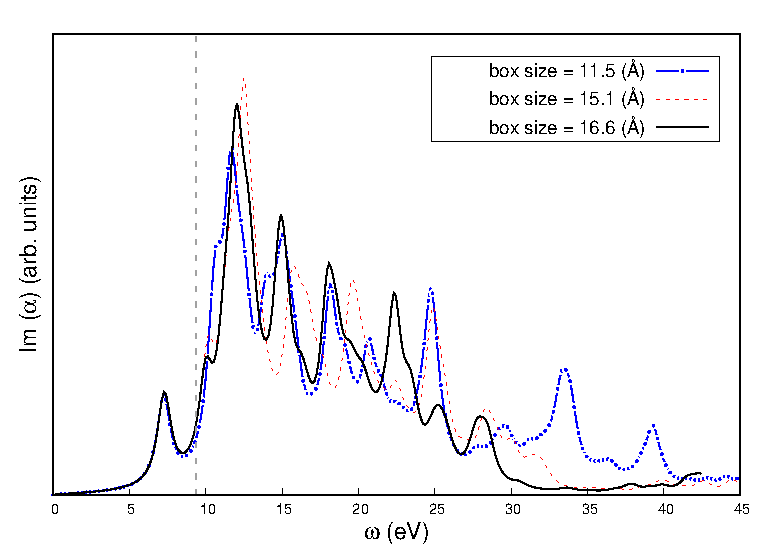
\includegraphics[scale=0.6]{CO_spectrum.eps}
\caption{\label{co_spectrum}(Color online) Convergence below threshold of the $CO$ spectrum computed in different computational setup.}
\end{figure}

Such concept of threshold has an evident physical interpretation: for energies in a range higher than the ionization potential,
localized and delocalized states might be coupled by the perturbation. Obtaining convergence of the observable quantities at these energies is therefore much more challenging if one employs 
numerical techniques which were originally tailored for GS calculations.

\section{Excitation operators. The analytic structure of the susceptibility functional}

In view of reproducibility, the scalar product of Eq.~\eqref{LinearResponseFunctDef1}, defining the observable fluctuation, may be compared among various numerical treatments.
However, even though directly related to experimental results, such quantity is not by itself a property of the molecule, as it is a function of $\omega$ that explicitly depends 
on the perturbation operator $\op \Phi$, not to mention the target observable $\op O$. Alternatively, we may consider only the fluctuation state, but it is still a $\op \Phi$-dependent wavefunction, 
%that may be local and with a well-defined normalization 
with a potential local behavior only for $\omega$ below the ionization threshold. Hence, comparing fluctuation states among diverse numerical treatments would be a 
challenging task.

It is therefore much more interesting to concentrate on LR quantities that are defined independently from the perturbing operators and target observables.
This can be achieved by studying the 
\emph{susceptibility functional}, defined implicitly trough the operator equation  
\be\lb{SusceptibilityDef1}
\dm'(\omega) = \left(\omega -\mathcal L \right)^{-1} \commutator{\op \Phi(\omega)}{\dmnot} = \sop{{\cal \chi}}(\omega) \op\Phi(\omega) \;. 
\ee
%This alternative formulation of the problem has the advantage of providing general information on the nature of the excitation spectrum. Results achieved in this way thus describes an intrinsic 
%feature of the system under inspection and determine the properties of the LR independently from the specific choice of the perturbing field. 
The susceptibility (super)operator $\cal \chi(\omega)$ is therefore closely related to the resolvent of the Liouvillian of Eq.~\eqref{LiouvillianRhopomegaDef1}, which is completely defined 
from the molecule hamiltonian $\hnot[\dm]$.
The ``excitation modes''  of the molecule are defined through the \emph{excitation operators}, satisfying
\be\lb{ExcitationOperatorsDef1}
\Liouv \op E_a = \Omega_a \op E_a \qq \op{\tilde E}_a \Liouv = \Omega_a \op{\tilde E}_a \;,
\ee
together with the operator orthonormalization condition %$\trace{\op{\tilde E}\op E'} = \delta(E-E')$. 
\be\lb{orthoExcitatioOpDef1}
\trace{\op{\tilde E}_a\op E_b} = \delta_{ab} \;.
\ee
Excitations defined in that way may be considered as a basis of the operators that satisfy the transverse condition as in  
Eq.~\eqref{RhopTransverseDef1}, and enable us to express the susceptibility as a spectral decomposition:
\be\lb{RhopExcitationDef1}
\sop{{\cal \chi}}(\omega) \cdot   = \sum_{\{a\}} \op E_{a} \,
\frac{\trace{\commutator{\op{\tilde E}_a}{\dmnot}\cdot}}{\omega-\Omega_a} \;.
\ee 

\subsection{The analytic structure of linear susceptibility}
Being themselves transverse operators, without loss of generality we can parametrize excitations by employing  
the \emph{excited states} $\ket{\phi^a_p}$ and $\bra{\chi^a_p}$ that, by construction, are orthogonal to the occupied orbitals
$\ket{\psi_p}$ and satisfy the normalization condition % and the orthonormalization condition \eqref{orthoExcitatioOpDef1} implies 
\be\lb{ExcitedStateOrthNormDef1}
\sum_p \left(\brket{\phi_p^a}{\phi_p^b} - \brket{\chi_p^b}{\chi_p^a}\right) = \delta_{ab} \;. 
\ee
In this way we can parametrize the excitation operators of the system as:
\begin{align}\lb{ExcitationOperatorsDef2}
\op E_a &= \sum_p \left( \ket{\phi^a_p}\bra{\psi_p} + \ket{\psi_p} \bra{\chi^a_p}\right)\;, \nn \\
\op{\tilde E}_a = \commutator{\dmnot}{\op E^t_a} &= \sum_p \left( \ket{\psi_p}\bra{\phi^a_p} - \ket{\chi^a_p} \bra{\psi_p}\right)\;.
\end{align}
Each excitation ``mode'' of the system $\op E_a$ with energy $\Omega_a$, can then be associated to a set of states $\{\phi^a_p,\chi^a_p\}_{p \in a}$,
entirely defined in the unoccupied subspace. For each choice of $p,a$, these objects represent, respectively, the state in which the occupied state $\ket{\psi_p}$
is excited -- or from whom it decays -- when the system is subject to the perturbation $\Phi_a \equiv \commutator{\dmnot}{\op E_a}$.
We denote with the shorthand $p \in a$ the fact that the sum of Eq.~\eqref{ExcitationOperatorsDef2}
is in general restricted only to a $a$-dependent subset of the occupied orbitals, depending on the particular symmetry 
of the excitation.

% We observe that right eigenvalues of $\Liouv$ can be written in terms of the left ones due to the properties 
% of the Liouvillian described in appendix \ref{LiouvillianAction}. 
% By applying equations \eqref{LiouZeroDef1},\eqref{CouplDef1} and \eqref{LiouvillianRightActionDef1} presented in 
% appendix \ref{LiouvillianAction} to the dyadic representations of the excitation 
% operators, 
By applying the equations \eqref{ExcitationOperatorsDef1} to the above parametrization
of the excitations, we obtain the following Sternheimer-like equations for the excited states:
\begin{align}\lb{ExcitationOperatorsDef3}
&\left[\Omega_a-(\hnot - \eps_p)\right] \ket{\phi_p^a} = \op Q_0 \op V'[\op E_a] \ket{\psi_p} \;, \nn\\
&\left[-\Omega_a-(\hnot - \eps_p)\right]\ket{\chi_p^a} = \op Q_0\op V'[\op E^t_a]\ket{\psi_p}  \;.
\end{align}
By writing these equations in a basis set of virtual states we obtain the well-known Casida's eigenvalue equation
associated to the excitation energy $\Omega_a$ (see appendix \ref{casida}).
The excitation spectrum is symmetric w.r.t the inversion of the eigenvalues 
$\Omega_a \rightarrow -\Omega_a$ and the associated excitation with negative energy are described by the transpose pair $\{\chi^a_p,\phi^a_p\}$.
We concentrate our analysis on the sector of positive energies, i.e. $\Omega_a > 0$.

With the same spirit of the previous sections, we present a formal solution of \eqref{ExcitationOperatorsDef3} as follows 
\begin{align}
\ket{\phi^a_p} &= \op G_H(\Omega_a+\eps_p)\left(\op V \ket{\phi^a_p} + \ket{s_{\phi}} \right) \;, \nn \\
\ket{\chi^a_p} &= \op G_H(-\Omega_a+\eps_p)\left( \op V \ket{\chi^a_p} + \ket{s_{\chi}} \right)\;,
\end{align}
where the source terms $s_\phi$ and $s_{\chi}$ are defined as:
\begin{align}
 \ket{s_{\phi}} &=  \op Q_0 \op V'[\op E_a] \ket{\psi_p} \nn \\
 \ket{s_{\chi}} &=  \op Q_0 \op V'[\op E^t_a] \ket{\psi_p}\;.
\end{align}
We first point out that the Helmholtz kernel associated to the $\ket{\chi^a_p}$ state 
contains an exponential damping factor for \emph{all} the positive values of $\Omega_a$.
The asymptotic long-range behaviour of $\ket{\chi^a_p}$ thus depends only on the locality properties of 
$\ket{s_{\chi}}$, which in turn is related to the behaviour of the operator $\op V'[\op E^t_a]$.
% As in the previous section, we assume the hypothesis that such operator is such that
% the state $\op Q_0 \op V'[\op E^t_a] \ket{\psi_p}$ is localized, at least when \emph{both}
% the states $\phi_p^a$ $\chi_p^a$ have bound-state-like behaviour.

On the other hand, the long-range behaviour of $\op G_H(\Omega_a+\eps_p)$ depends from 
$\Omega_a$, with a threshold of value $\Omega_a=|\eps_p|$. 
For energies above this value, the behaviour of the state $\ket{\phi^a_p}$ is 
delocalized regardless of the particular nature of the operators $\op V$ and $\op V'$.
This means that, if an excitation operator $\op E_a$ has an energy such that
$\Omega_a>|\eps_p|$  for \emph{at least one} of the $p \in a$ defining the excitation,
such operator cannot be parametrized by employing localized states only.

As a consequence, we deduce that a molecular excitation \emph{may} be expressed in terms of localized states
\emph{only} when its energy is lower than \emph{all} the ionization potentials of the occupied states participating to the excitation,
namely if $\Omega_a<|\eps_p|$ $\forall p \in a$. This will only be true if the operators
$\op V'[\op E^t_a]$ and $\op V'[\op E_a]$ can be restricted to localized wavefunctions.
If any of these hypothesis does not hold, the excitations of the systems are defined via genuinely delocalized wavefunctions.
% As a consequence of these behaviors and assuming the spatial localization of 
% the source terms,  we observe that the asymptotic character of $\ket{\phi^a_p}$ changes from bound to unbound as the value of the excitation energy crosses the threshold $|\eps_p|$ while all 
% the $\ket{\chi^a_p}$ states exhibit a bound-state behavior for all the values of $a$. 
Furthermore, excited states are subjected to the orthonormalization condition 
\eqref{ExcitedStateOrthNormDef1} that acts as a ulterior constraint and has the effect of determining the \emph{quantization}
of the energy levels $\Omega_a$ associated to the bound-state-like objects.
For delocalized states, as in the case of the continuum states of $\hnot$,
such a condition has to be interpreted in disctributional sense and does not lead to quantization of $\Omega_a$.
Thus we can conclude that all the states $\ket{\chi^a_p}$ and the $\ket{\phi^a_p}$ with $\Omega_a$ below the threshold value constitute 
-- if localized -- a genuine \emph{discrete} set, while the ones in the unbound energy range behaves as generalized eigenvectors associated to a
continuum spectrum. 

%%%%%%%%%%%%%%%%%%%%%%%%%%%%%%%%%%%%%%%%%%%%%%%%%%%%%%%
\begin{figure}[!t]
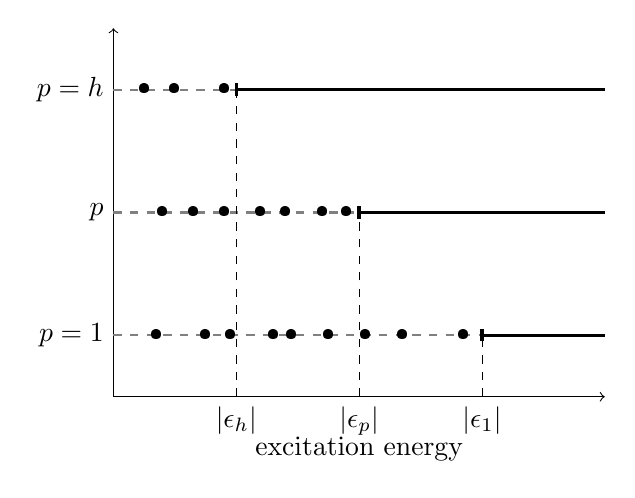
\begin{tikzpicture}[scale=0.78]
% axes
\draw[->] (0,0) -- (8,0); 
\draw[->] (0,0) -- (0,6);
% orizontal lines
\draw[dashed,thick,color=gray] (0,5) -- (2,5);
\draw[very thick](2,5) -- (8,5);
\draw[dashed,thick,color=gray] (0,3) -- (4,3);
\draw[very thick] (4,3) -- (8,3);
\draw[dashed,thick,color=gray] (0,1) -- (6,1);
\draw[very thick] (6,1) -- (8,1);
% % vertical lines
\draw[dashed,very thin,color=black] (2,0) -- (2,5);
\draw[dashed,very thin,color=black] (4,0) -- (4,3);
\draw[dashed,very thin,color=black] (6,0) -- (6,1);
% % threshold levels labels
\node[left] at (0,5) {$p=h$};
\node[left] at (0,3) {$p$};
\node[left] at (0,1) {$p=1$};
\node[below] at (2,0) {$|\eps_h|$};
\node[below] at (4,0) {$|\eps_p|$};
\node[below] at (6,0) {$|\eps_1|$};
\node[below] at (4,-0.5) {excitation energy};
% bars at thresholds
%\foreach \Point in {(2,5),(4,3),(6,1)}{
%   \node at \Point {{\textbar}};%$\times$};
%}
\draw[very thick] (2,4.9) -- (2,5.1);
\draw[very thick] (4,2.9) -- (4,3.1);
\draw[very thick] (6,0.9) -- (6,1.1);
% dotted vertical lines
%\draw[dotted,thick,color=black] (-0.2,3.6) -- (-0.2,4.4);
%\draw[dotted,thick,color=black] (-0.2,1.6) -- (-0.2,2.4);
% discrete excitations
\foreach \Point in {(0.5,5),(1.0,5),(1.8,5),(0.8,3),(1.3,3),(1.8,3),(2.4,3),(2.8,3),(3.4,3),(3.8,3),(0.7,1),(1.5,1),(1.9,1),(2.6,1),(2.9,1),(3.5,1),(4.1,1),(4.7,1),(5.7,1)}{
    \node at \Point {\textbullet};
}
\end{tikzpicture}
\caption{\label{ExcitationLandscape} Excitation landscape. Excitation are split in horizontal line according to the threshold levels $p_m$. Filled bullet refers to localized
excitations whereas the tick black lines describe delocalized excitation with a continuum spectrum.}
\end{figure}
%%%%%%%%%%%%%%%%%%%%%%%%%%%%%%%%%%%%%%%%%%%%%%%%%%%%%%%

% The structure of the excitation spectrum follows from the properties of the excited states described above. 
% To clarify this point we consider a value of $\Omega_a$ that satisfies equations
% \eqref{ExcitationOperatorsDef1}. In correspondence of this values equations \eqref{ExcitationOperatorsDef3} 
% possess a solution in which \emph{at least} one of the excited states 
% is not zero. We denote with $p=p_m$ the label of the $\ket{\phi^a_p}$  with the highest value of $|\eps_p|$, among the ones that contribute to \eqref{ExcitationOperatorsDef2}. From the previous 
% considerations it emerge that if $\Omega_a<|\eps_{p_m}|$ \emph{all} the excited states in the dyadic representation of the excitation operator possess a bound-state like behavior. Excitations 
% of this type thus represent localized quantities and the associated eigenvalue are discrete. On the contrary, for $\Omega_a>|\eps_{p_m}|$ some (or all) of the excited states in the dyadic representation
% of the excitation behave as generalized eigenvectors and the corresponding eigenvalue belong to a continuum of accessible values.

The susceptibility functional has therefore a peculiar analytic structure, that
is made of multiple threshold energies, one for each of the ionization potentials
associated to the occupied states. 
If an excitation $\op E_a$ has a energy $\Omega_a < |\eps_a|$ with $\eps_a = \mathrm{max}\left(\eps_p\right)_{p\in a}$,
it may belong to a discrete spectrum; otherwise it \emph{has} to belong to a continuum of states. 

Following these observations, the typical structure of the excitations landscape is depicted in figure \ref{ExcitationLandscape}, once again assuming a reasonable 
behavior of the perturbed potential $\op V'$.
Below the first ionization energy $|\eps_h|$ only localized excitations are present. Conversely, in the intermediate energy interval that extends from $|\eps_h|$ to the 
absolute value of the deepest occupied orbital, other discrete excitations may exist, and are embedded in a continuum of delocalized excitations. 
Lastly, for energies higher than $|\eps_1|$ \emph{no localized} excitations are anymore possible,
regardless of the particular behavior of $\op V'$ so the excitations landscape in this region is composed only by continuum energies.

\subsection{Observable features of the excitation spectrum}
%\subsection{Stability and convergence of the excitation spectrum}

The analysis of the above section reveals that the excitation spectrum is composed by two distinct sectors. 
The first one is realized by the (finite) set of localized excitations with discrete eigenvalues. 
% Extending the results achieved in \cite{boffi2016} for the KS virtual orbitals, 
%to the equations for excited states 
%\eqref{ExcitationOperatorsDef3}, we conclude that such localized excitations behave as 
Borrowing the terminology introduced in section \ref{SEopenSystem} to the present case, we can affirm that such localized excitations behaves as
\emph{observable} quantities and the associated energies possess ideal features of reproducibility:
if the numerical basis employed is complete enough to
represent the states $\{\phi_p^a,\chi_p^a\}$, the energy $\Omega_a$ 
should not depend from the computational setup used for their representation.

Instead, the second sector contains the dense set of delocalized excitations with an associated continuum spectrum. These excitations behave as the unbound virtual orbitals analyzed in \cite{boffi2016} 
and are deeply affected by the computational setup used to represent them. In particular, the presence of a finite computational domain implies a fictitious discretization of the excitation levels and 
the associated spectrum exhibit an explicit dependence from the size of the domain. 
Excitations belonging to this sector thus lose their intrinsic physical meaning and have to be understood simply as
a representation of the density of states of the Liouvillian superoperator.

\begin{figure}[ht]
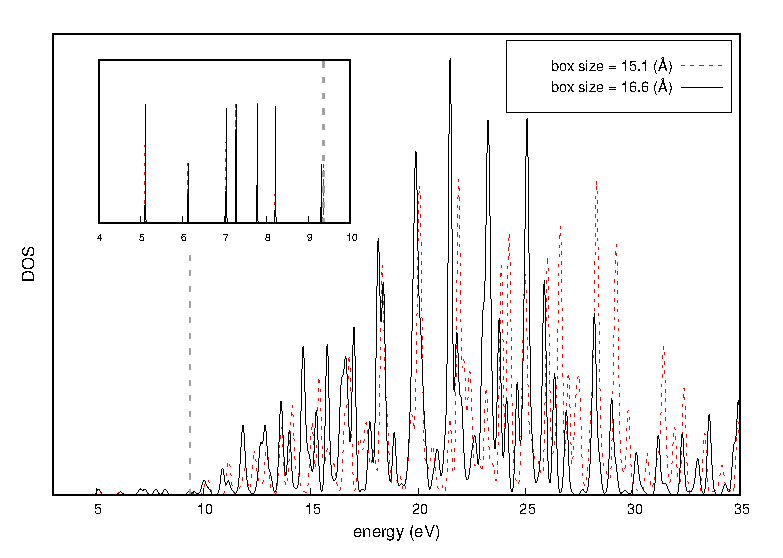
\includegraphics[scale=0.6]{CO_dos.eps}
\caption{(Color online) Excitation spectrum of $CO$. The two curves correspond to two computational domain of different sizes. The inset contains the sole contribution of localized excitations.}
\label{CO_exc}
\end{figure}
\begin{figure}[ht]
\centering
\subfloat[aaaa]
{\label{c6h6_excLand}
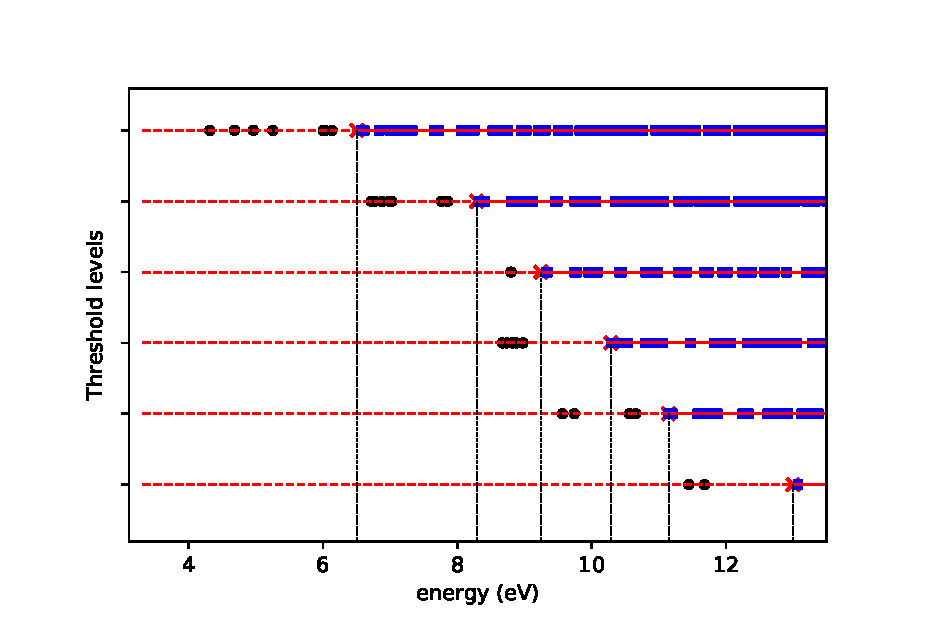
\includegraphics[scale=0.56]{C6H6_excLandscape.eps}} \\
\centering
\subfloat[bbbbb]
{\label{C6H6_exc}
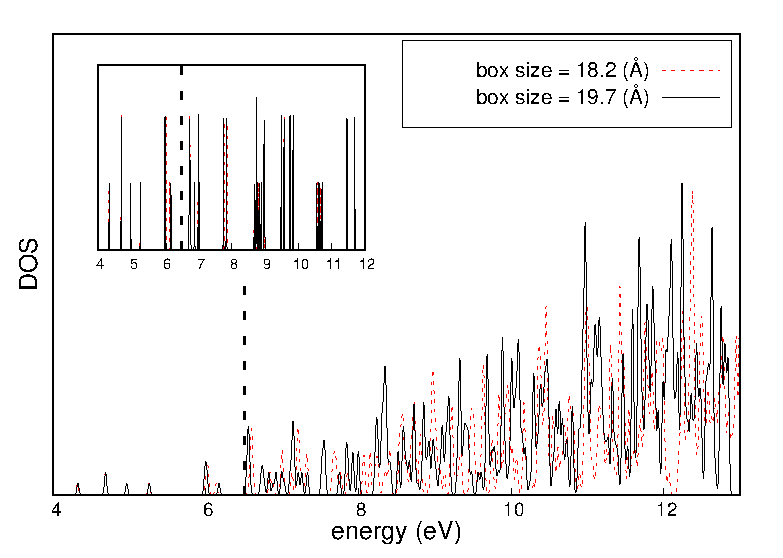
\includegraphics[scale=0.58]{C6H6_dos.eps}}
\caption{(Color online) Excitation landscape and DOS of $C_6H_6$.}
\end{figure}


In Fig.~\ref{CO_exc} and \ref{C6H6_exc} we plot the Density of States of the Liouvillian for the $CO$  and Benzene molecules, 
for two different numerical setups of increasing simulation domains. 
The figures show clearly that all the excitations of energy $\Omega_a$ lying below the 
molecule ionization potential (IP) have a clear localized behaviour, as their energy does not vary with the size of the simulation domain.
On the other hand, above the first ionization threshold the excitation energies have an energy that strongly depends on the computational
setup, which is in line with the expected pseudo-continuum character of this sector. 
In addition, for the benzene molecule it is also possible to 
identify excitations of energy above IP that still possess a localized behaviour: these excitations satisfy the
condition $\Omega_a < |\eps_a|$ presented in the above section.
In Fig.~\ref{c6h6_excLand} we collect the excitations of the benzene molecule following this criterion:
the agreement with the expected analytic structure presented in Fig.~\ref{ExcitationLandscape} is remarkable.


%\subsection{The importance of the continuum sector}
\subsection{Physical relevance of the continuum sector}

We have presented formal arguments, confirmed by numerical calculations, that show that 
the excitations belonging to the discrete sector of the spectrum have energies
that can be \emph{quantitatively} compared between codes, thanks to their
localized character. 
Such objects are LR quantities, associated to the molecule, whose numerical convergence
can be found by employing techniques which are very similar to 
the one adopted for GS calculations. Being expressed by localized excited states,
computational setups with sufficient level of completeness are able to
express with high \emph{precision} such section of the excitation spectrum.

It is interesting to obtain information on whether such localized excitations
will be sufficient to express LR quantities that are associated to localized
fluctuation states.
By recalling that $\ket{f_p^\Phi(\omega)} = \dm'_\Phi(\omega) \ket{\psi_p}$,
considering Eq.~\eqref{SusceptibilityDef1} and
expressing the spectral decomposition of the linear susceptibility we find:
% \begin{align}
%  \ket{f_p^\Phi(\omega)} &= \ket{f^\Phi_p(\omega)^D} + \ket{f^Phi_p(\omega)^C} \lb{FSExcitationDef1} \\
%  \ket{f_p^\Phi(\omega)^D} &= \sum_a^{0<\Omega_a < |\eps_a|} \ket{w_p^a} \frac{f_p^a(\op \Phi,\omega)}{\omega^2-\Omega_a^2} \\
%  \ket{f_p^\Phi(\omega)^C} &= \int_{0<\Omega_a > |\eps_a|} \!\!\!\!\dd a \ket{w_p^a} \frac{f_p^a(\op \Phi,\omega)}{\omega^2-\Omega_a^2}
% \end{align}
\be
\ket{f_p^\Phi(\omega)} = \fscd{D} + \fscd{C}
\lb{FSExcitationDef1} \;,
\ee
with
\begin{align}
 \fscd{D} &= \sum_a^{\Omega_a < |\eps_a|} \ket{w_p^a} \frac{\varphi_p^a[\op \Phi(\omega)]}{\omega^2-\Omega_a^2} \;, \nn \\
 \fscd{C}
 &= \int_{\Omega_a > |\eps_a|} \!\!\!\!\dd a \ket{w_p^a} \frac{\varphi_p^a[\op \Phi(\omega)]}{\omega^2-\Omega_a^2} \;, \nn
\end{align}
where $\varphi_p^a[\op \Phi(\omega)] \equiv \bra{\psi_p}\op\Phi(\omega)\ket{w_p^a}$,
and $\ket{w_p^a}=\ket{\phi_p^a}+\ket{\chi_p^a}$. 
In the above equation we have explicitly separated the contributions of the discrete ($D$) and continuous ($C$) excitations 
in the spectral decomposition \eqref{SusceptibilityDef1}.
The summation and the integration run only on the positive values of $\Omega_a$.
The states $\ket{w_p^a}$ that appear in the discrete sum 
or in the integral are genuinely localized and delocalized, respectively.
For \emph{any} value of $\omega$ the ket $\fscd{D}$ has, by definition, a bound-state like
character as it is expressed as a sum of localized contributions.

We have seen in Sec.~\ref{FluctuationState} that 
for values of $\omega$ below the first ionization potential we expect
$\ket{f_p^\Phi(\omega)}$ to have bound-state like behavior.
However, there is no particular reason to believe that $\fscd{C}$ should be
zero. Since $\ket{w_p^a}$ states are linearly independent, 
$\fscd{C}=0$ would imply
$\varphi_p^a[\op \Phi(\omega)]=0$ for any $a$ labelling the continuum excitations,
which is too strong a condition for a general choice of $\op \Phi$
\footnote{The plot in Fig.~\ref{co_AlphaExc}
show this evidence even in the simple case when $\op \Phi$ is the dipole operator.}.
Therefore,  the contribution from the delocalized excited states defining
$\fscd{C}$ should resum into a localized, asymptotically vanishing state.

This means that, contrary to GS, \emph{for LR calculation,
even when the response density is localized, the contribution coming from the 
continuum sector of the excitations can never be neglected}. 
In other terms, we \emph{cannot} exclude that a fluctuation state, even if genuinely localized, will have a nonzero projection
in the essential part of the Liouvillian spectrum.

\begin{figure}
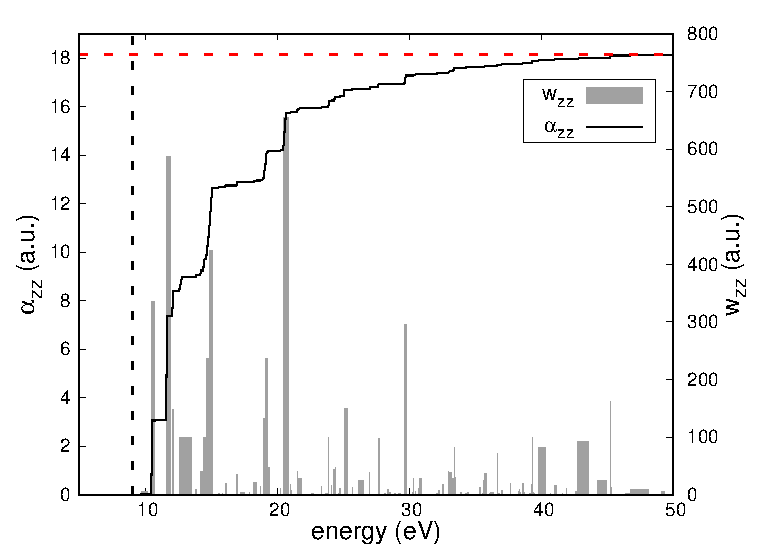
\includegraphics[scale=0.6]{CO_statPolvsExc.eps}
\caption{\label{co_AlphaExc}(Color online) Convergence of the statical polarizability of the $CO$ molecule w.r.t the number of excitations.}
\end{figure}
We show an evidence of the above statement in Fig.~\ref{co_AlphaExc}. Indeed,
we may decompose the linear response functional of Eq.~\eqref{LinearResponseFunctDef1}
for any operator $\op O$ as $\braket{\delta\op O}_\Phi=\braket{\delta\op O}^D_\Phi +
\braket{\delta\op O}^C_\Phi$, where
\be
\braket{\delta\op O}^{D,C}_\Phi(\omega) = 
2 \mathrm{Re}\left(\bra{\psi_p} \op O \fscd{D,C} \right)\;.
\ee
The static polarizability tensor $\alpha_{ij}$ can be easily expressed
from the above quantities as
\be
\alpha_{ij} = \sint \dd a \frac{w^a_{ij}}{\Omega_a^2}\,, \quad w^a_{ij} \equiv \sum_{p\in a} \varphi_p^a[\op r_i]\varphi_p^a[\op r_j]\;.
\ee
The above relation shows that the value of $\alpha_{ij}$ explicitly depends on the set of excitations
included in the integral defining $\fscd{C}$.
+Such value can be straightforwardly compared with results of Eq.~\eqref{staticalpha}, where the localized FS is obtained from GS techniques as described in Sec.~\ref{FluctuationState}.
This is the well-know $S_{-2}$ sum-rule\cite{TDDFTBOOK}, that express the value of the static polarizability
in terms of the molecule's oscillator strengths.

We see that a considerable number of pseudo-continuum excitations is required
to find the correct result; the sector of the discrete excitations, even though 
parametrised by localized, observable (in the sense of reproducible) excited states,
appears to be largely insufficient to express the reference fluctuation state.
This seems to be independent on the number of atoms of the molecule, as the range in $\omega$ needed to 
achieve satisfactory agreement is largely above the last valence ionization threshold, which is
a intensive (i.e. independent on the number of atoms) quantity.
The inclusion of core electrons in the calculation would have added a further set of localized
excitations, but at much higher energies than the one needed for this test.

This fact shows that it is \emph{impossible} to restrict the spectral representation
of $\chi(\omega)$ only localized and discrete excitations, even for representing LR results in the $\omega=0$ limit.
In addition, we can see that the above sum-rule \emph{cannot} be used to assess
the correctness of $\chi(\omega)$ for values of $\omega$ above IP; it is enough to recall
the strong dependency on the box size of the absorption spectra of Fig.~\ref{CO_exc}.
For all these computational setups, the $S_{-2}$ sum rule is, on the contrary, perfectly satisfied.

\section{Conclusions and Perspectives}
% In the analysis presented in this paper we have investigated how 
% computational results of linear-response calculations of molecular systems 
% might be compared among various formalisms.
% In particular, we have been interested in identifying the quantities that can
% be expressed in computational setups that are originally conceived for 
% \emph{localised} objects, which are the \emph{only} quantities that
% play a significant role in GS calculations.

By analysing the fundamental equations of LR calculations of molecules, we have shown that the response density for values of $\omega$ above the first IP
\emph{have} to be expressed in terms of genuinely delocalized states. %, whereas 
Below this threshold,
under reasonable assumptions on the perturbing operators,
the perturbed density operator is genuinely localized.
In this localized regime, it is possible to achieve convergence of the numerical result
by increasing the completeness of the basis with the usual GS rationales.
One might expect that more complete basis will give more precise results, regardless of their asymptotic behavior.
A comparison among various codes in view of reproducibility should therefore be performed 
initially in this regime.

The situation is not so simple in the above-threshold regime.
In this case what is important is the matrix element of the observable of interest
between the bound, occupied state and the fluctuation state (FS). 
The FS is here an unbound, delocalized function, and a numerical treatment tailored for localized functions will \emph{never} be able to discretise such function with arbitrary accuracy.  
To achieve numerical convergence, care should be taken in expressing accurately the FS on the
appropriate region of space. In view of reproducibility, computational setups which are able to express precisely
delocalized states seem more interesting in this regime.

Such point of view have also enabled us to shed light on the analytic structure of the 
linear susceptibility, which is a intrinsic property of the molecule and does not depend on
 the perturbing fields.
 In particular, we have concentrated our interest in its spectral representation in
 terms of ``free oscillation'' (i.e. excitations) of the system.
 We have found that \emph{not all} the excitations have to be considered on equal footing.
 As the excitation spectrum has several energy thresholds, one per quasi-particle IP,
 there is a sector of \emph{discrete}, \emph{localized} excitations -- whose energies are 
below the corresponding threshold -- which can be compared among different computational treatments.
Their energies are \emph{true} poles of the linear susceptibility, the excited states being their residues.

On the other hand, the excitation energies which lie above these thresholds are only pseudo-poles of $\chi(\omega)$, 
and will \emph{strongly} depend on the computational setup. This is visible for energies higher than
IP, and it has been pointed out several times (see e.g. \cite{giustino2012,giustino2014}) in the literature.
These excitations belong to a continuum sector that embeds the above mentioned discrete excitations.
We remark that we are not referring here to the continuum eigenstates of the 
unperturbed GS hamiltonian, %which is not in itself important for expressing the linear susceptivity, 
but to the continuum of excitations expressed as eigenstate of the 
Liouvillian superoperator of Eq.~\eqref{LiouZeroDef1}, needed to 
express the spectral representation of the linear susceptibility.

Both the sectors of the excitations energies have to be considered in view of the extraction of computationally reliable quantities.
We can \emph{quantify} the reliability of excitations belonging to the discrete sector, as the corresponding excited states and energies may be discretized with arbitrary accuracy on a localized region.
For instance, absorption spectra \emph{below IP} are relatively easy to converge, as they are observables which depend only on localized quantities.

We are, on the contrary, forced to provide effective representations for
the delocalised excitations belonging to the (pseudo-) continuum sector.
For generic LR quantities, which are functionals of the linear susceptivity, 
the quality of the $\chi(\omega)$ (super)operator will depend
on the frequency $\omega$ of interest: a given spectral representation may provide high-quality results for static $\omega=0$ regimes, while being
unable to provide convergence for high-energy absorption spectra.

% As an illustration, we have presented explicitly examples where the pseudo-contunuum sector is relevant: in the same 
% We have shown computational setups in which convergence difficulties high-energy absorbption spectra are observed, whereas the $S_{-2}$ sum rule (meaningful in the $\omega=0$ regime) is precisely fulfilled.

% However, this does not necessarily imply that for $\omega$ above thresholds 
% the same pseudo-continuum expansion can be effectively employed: we have shown spectral representation of $\chi(\omega)$ which presents difficulties in convergence of high-energy absorbption spectra, whereas they provide precise values of the excitation energies in the discrete sector.
% In other terms, the set of continuum excitations may only be \emph{effectively} represented
% in a computational approach, depending on the quantities of interest.

We believe that these considerations, based on simple manipulations on the fundamental LR equations, will help in increase
the reliability of LR calculations in the community, and in building test-sets that would help in
the \emph{calibration} of present and future computer codes, thereby increasing the predictivity of present-day theoretical approaches.
The example of the static polarizability of molecules
presents ideal features as an initial playground. Work is ongoing in this direction.


% \section{Garbage Collector}

%The introduction of the excitation operators allows us to express the spectral decomposition of the resolvent of the Liouvillian so that:
%Susceptibility written as
% The introduction of the excitation operators allows us to express the susceptibility functional \eqref{SusceptibilityDef1} through the spectral decomposition of the resolvent of the 
% Liouvillian. Pursuing this procedure provides:
% \be\lb{RhopExcitationDef2}
% \sop{{\cal \chi}}(\omega) \cdot   = \left(\sum_a + \int\dd a   \right) \op W_{a} \,
% \frac{2\trace{\op W_a \cdot}}{\omega^2-\Omega_a^2} \;,
% \ee 
% where we have defined the symmetric operators $\op W_a = \frac{1}{\sqrt{2}}(\ketbra{w_p^a}{\psi_p}+\ketbra{\psi_p}{w_p^a})$ and states $\ket{w_p^a}=\ket{\psi_p^a}+\ket{\chi_p^a}$.


% The elements of the first category correspond to \emph{true poles} of the susceptibility while the others can be interpreted only in terms of the spectral function. 

% This analysis has revealed that the excitations spectrum is composed by two distinct sectors. The first one is realized by the (finite) set of localized excitations with discrete eigenvalues. Extending 
% the results achieved in \cite{boffi2016} for the KS virtual orbitals, to the equations for excited states \eqref{ExcitationOperatorsDef3}, we conclude that localized excitations behave as 
% \emph{observable} quantities and the associated energies possess an absolute meaning, which should not depend from the computational setup used for their representation. 
% 
% Instead, the second sector contains the dense set of delocalized excitations with an associated continuum spectrum. These excitations behave as the unbound virtual orbitals analyzed in \cite{boffi2016} 
% and are deeply affected by the computational setup used to represent them. In particular, the presence of a finite computational domain implies a fictitious discretization of the excitation levels and 
% the associated spectrum exhibit an explicit dependence from the size of the domain. Excitations belonging to this sector thus lose their intrinsic physical meaning and have to be understood as a tool to 
% express the spectral decomposition of the Liouvillian superoperator. 



% Lastly, we establish a link between the fluctuation states and excitation operators based description of the LR. Indeed, thanks to the defining equation \eqref{SusceptibilityDef1} we can 
% easily express the excitations expansion of fluctuation states as follows 
% \be\lb{FluctuationStateExcitationDef1}
% \ket{f_p(\omega)}   =
% \left(\sum_E + \int\dd E   \right) 
% %\frac{\trace{\commutator{\dmnot}{\op{\tilde E}}\op\Phi(\omega)}}{\omega-E} \ket{\phi^E_p} \;. \nn
% \frac{t_\Phi(E)}{\omega-E} \ket{\phi^E_p} \;,
% \ee 
% with $t_\Phi(E)=\trace{\commutator{\dmnot}{\op{\tilde E}}\op\Phi(\omega)}$. 
% %This formula shows that, for each value of $\omega$, both the sectors of the excitations spectrum contribute to the fluctuation state. 
% Thanks to the analysis presented in section \ref{FluctuationState} we know that fluctuation states possess a localized behavior up to $\omega=|\eps_h|$, so we conclude that 
% below this energy threshold the continuum sector of the excitation spectrum is able to resum in a localized way.  


%Excitations behave as singularity of the susceptibility operator and their knowledge provides a deeper insight into the analytic structure of the linear response. 

%\subsection{Discrete poles and spectral function. Physical meaning of the excitation spectrum} %{Comments. Physical meaning of the excitation spectrum}

% The analysis discussed above has evidenced that there exists both localized and delocalized excitations. While the role of the former is quite unambigous 
% We can express the 
% \be\lb{FluctuationStateExcitationDef1}
% \ket{f_p(\omega)}   =
% \left(\sum_E + \int\dd E   \right) 
% %\frac{\trace{\commutator{\dmnot}{\op{\tilde E}}\op\Phi(\omega)}}{\omega-E} \ket{\phi^E_p} \;. \nn
% \frac{t_\Phi(E)}{\omega-E} \ket{\phi^E_p} \;,
% \ee 
% with $t_\Phi(E)=\trace{\commutator{\dmnot}{\op{\tilde E}}\op\Phi(\omega)}$.
% This relation clarifies the role of the excitations in the spectral decomposition. We know from the analysis of section \ref{FluctuationState} that fluctuation states are localized
% up to $\omega=|\eps_h|$. 

%\section{Quality indicator for the numerical convergence of the LR}   %{Criterion for a reliable sampling of the excitation operators}

% From the analysis discussed in the previous section it emerges that the general treatment of the LR for open systems \emph{requires} to deal with delocalized
% objects. In facts, either if one choose the fluctuation states' formalism, or the ``sum over excitations'' (SOE) approach, it turns out that the main building blocks
% beyond a specific energetic threshold have an unbound behavior in the long range. 
% On the basis of this consideration is then reasonable to try to understand if a computational setup tailored to deal with the ground state problem is idoneous to provide
% reliable results for the LR. 

% \vspace{0.3cm}



% \begin{figure}[ht]
% 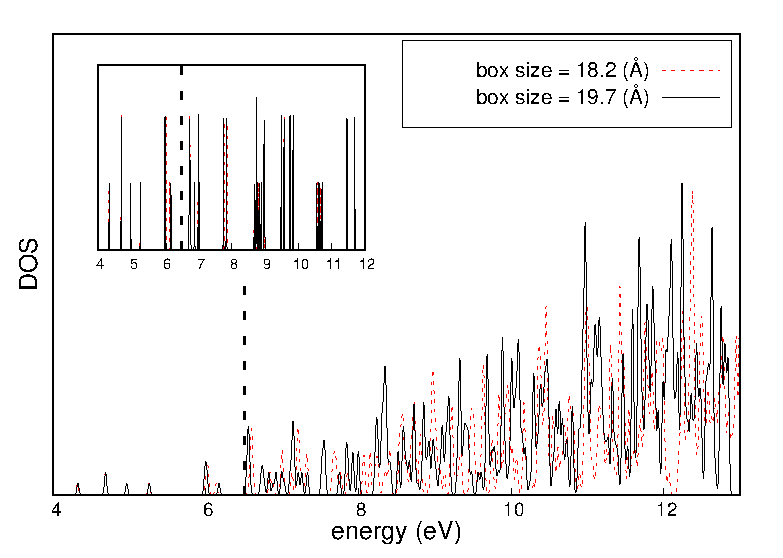
\includegraphics[scale=0.6]{C6H6_dos.eps}
% \caption{(Color online) Excitation spectrum of $C_6H_6$. The two curves correspond to two computational domain of different sizes. The inset contains the sole contribution of localized excitations.}
% \label{C6H6_exc}
% \end{figure}
% 
% \begin{figure}[ht]
% 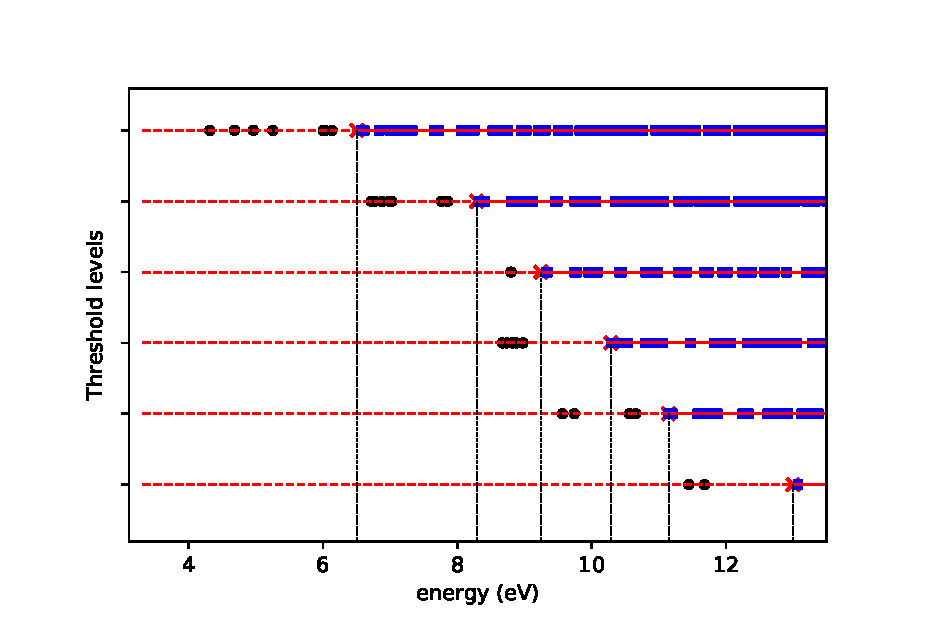
\includegraphics[scale=0.56]{C6H6_excLandscape.eps}
% \caption{\label{c6h6_excLand}(Color online) Excitation landscape of $C_6H_6$.}
% \end{figure}

% \begin{figure}[ht]
% \centering
% \begin{subfigure}[]{0.2\textwidth}
% 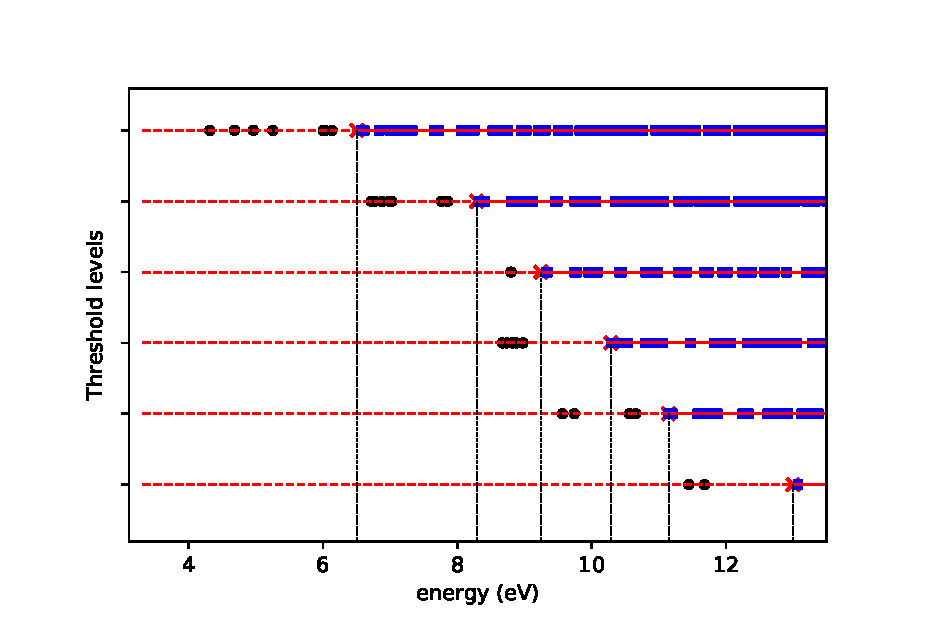
\includegraphics[scale=0.56]{C6H6_excLandscape.eps}
% %\caption{\label{c6h6_excLand}(Color online) Excitation landscape of $C_6H_6$.}
% \end{subfigure}
% \centering
% \begin{subfigure}[b]{0.2\textwidth}
% 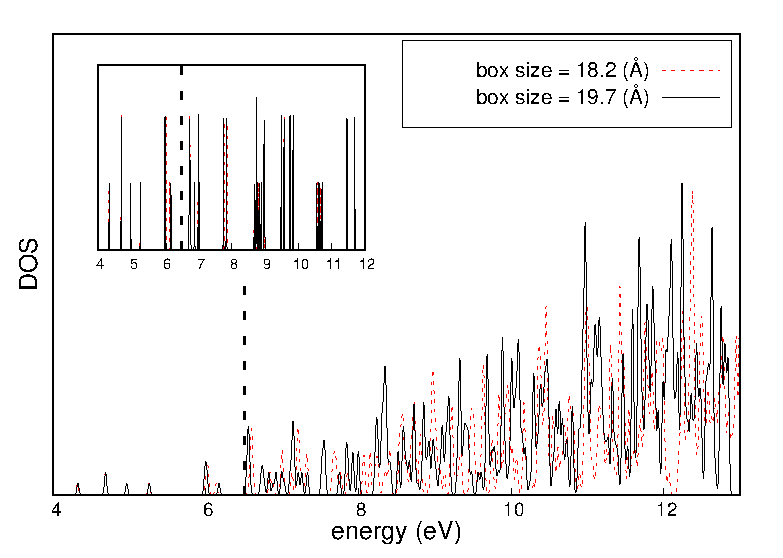
\includegraphics[scale=0.6]{C6H6_dos.eps}
% \end{subfigure}
% \caption{(Color online) Excitation spectrum of $C_6H_6$. The two curves correspond to two computational domain of different sizes. The inset contains the sole contribution of localized excitations.}
% \end{figure}

% From the theoretical analysis of the previous section we can made two statements:
% \begin{itemize}
%  \item Fluctuation states, which constitute the building blocks of the response density, have a bound state-like character up to $\omega=|\eps_h|$ and behave as unbound delocalized
%  wave functions for higher values of $\omega$. 
%  \item The excitation landscape is composed of two sectors with distinct properties. The elements of the first one behave as localized, observable quantities and contribute as discrete 
%  poles to the spectral decomposition of the susceptibility functional. The second sector contains a continuum of delocalized excitations which represents a tool to provide
%  an effective representation of the spectral function. 
% \end{itemize}
% The topic to be discussed in this section is the following: on the basis of these statements can we define some indicator to evaluate the reliability of a linear response calculations? And, 
% if so, up to which energy threshold can we assume that our computations do converge?
% 
% The first element of this discussion is the introduction of the computational basis, made of $n_\mu$ basis functions $\{\mu\}$, used to perform the DFT calculations subjacent to the LR analysis. 
% The properties of the $\mu$-basis (state something about the systematic character the basis? comment on the finite dimension of the computational domain?) are chosen to ensure an unbiased description 
% of the ground state properties of the system. 
% 
% FIRST QUESTION: The usage of the $\mu$-basis allows us to obtain a reliable evaluation of the perturbation induced modification of an observable? 
% The answer of this question is based on the analysis of equation \eqref{LinearResponseFunctDef2} and has been partially provided in section \ref{FluctuationState} (move that material in this section?). 
% We can complete the answer by observing that $\ket{f_p(0)}$ can be obtained through a ground state calculation with the explicit time independent perturbation added to the system. So we can perform
% a check on the goodness of the basis in this case as in a ground state calculation. Then use the localization argument of the fluctuation states to extend the reliability of the result up to
% $\omega=|\eps_p|$. 
% 
% SO TO SUMMARIZE: below the threshold the numerical convergence is regulated by the localization of the fluctuation states, in this range we can assess the reliability of the results provided by
% the $\mu$-basis by looking at the basis-independence of the fluctuation states at $\omega=0$. Above the threshold the convergence can be reached due to the localized nature of $\bra{\psi_p}\op O$, 
% in this case the computational setup provides reliable results if it guarantees the unbiased reconstruction of fluctuation states in the support of $\bra{\psi_p}\op O$. In this range there is no a 
% priori indicator of the goodness of the results. 


% \subsection{Fluctuation state and excitations}

% Show the convergence of the statical polarizability of the $CO$ in function of the number of excitations. Write formula
% \be\lb{AlphaExcitationDef1}
% \alpha_{xx} =  \left(\sum_a + \int\dd a   \right) 2 \,
% \frac{\left[\trace{\op W_a \op X}\right]^2}{\Omega_a^2} \;,
% \ee 
% and add the plot that show the convergence rate of the statical polarizability to the reference (finite difference) value in functions of the number of excitations. The plot evidence that the
% continuum sector of the excitation spectrum is 

% \subsection{Choice of the $\alpha$-basis. Statical polarizability-driven criterion revised}
% 
% The previous considerations regard the relation between the localization properties of the fluctuation states and the possibility of having a quality indicator for the goodness of the $\mu$-basis. 
% Now we aim to extend/reformulate the question of the numerical convergence to the case in which the excitation-based representation of the LR is adopted.
% 
% The construction of the excitation operators requires the explicit sampling of the empty state subspace. We introduce the notion of \emph{$\{\alpha\}$-basis}: choose the empty eigenstates of the KS 
% Hamiltonian as a basis-set to express the excited state $\ket{\phi^E_p},\bra{\tilde\chi^E_p}$ and their duals. Excitations are written in the basis of transitions.  
% 
% COMMENT: The elements of the $\{\alpha\}$-basis are written in the (finite dimensional) $\{\mu\}$-basis. It follows that the $\{\alpha\}$-basis is finite dimensional too and has $n_\mu-n_{occ}$ degrees
% of freedom. Excitation index becomes discrete and the basis provide a partial sampling of the continuum sector of the excitation landscape.    


% \subsection{Comments and conclusions}

% The analysis carried out starting from the representation of the linear response functional in terms of fluctuation states has evidenced some general properties of the linear response
% for open systems. In particular, by analyzing the asymptotic behavior of fluctuation states in long range limit, we have showed that they exhibit a bound-state character in the regime  
% $\omega<|\eps_h|$. Consequently we have argued that the linear response functional, in the same $\omega$ range, provides a setup-independent result with a modest computational effort... 



\appendix
\section{Transverse operators and right action of the Liouvillian superoperator}\lb{LiouvillianAction}
Given a unperturbed Hamiltonian and density operator, which satisfy $\commutator{\hnot}{\dmnot}=0$, we may decompose a generic operator in two contributions, $\op O=\op O_\parallel + \op O_\perp$, defined as:
\begin{align}
\op O_\parallel &\equiv \dmnot \op O \dmnot + \op Q_0 \op O \op Q_0 \nn \;,\\
\op O_\perp &\equiv \dmnot \op O \op Q_0 + \dmnot \op O \op Q_0 = 
\commutator{\dmnot}{\commutator{\dmnot}{\op O}} \;,
\end{align}
with $\op Q_0 =\identity - \dmnot$.
The operator $\op O_\parallel$ is constructed to satisfy 
$\commutator{\dmnot}{\op O_\parallel} = \commutator{\hnot}{\op O_\parallel} =0$.
Also, it is easy to verify that given two generic $\op O$, $\op O'$, we have
$\trace{\op O'_\parallel \op O_\perp} =0$.

The projection $\op O_\perp$ is therefore the relevant part for the commutator:
\begin{equation}
\commutator{\dmnot}{\op O} = \commutator{\dmnot}{\op O_\perp} =
\dmnot \op O \op Q_0  - \dmnot \op O \op Q_0 \;.
\end{equation}
The Liouvillian superoperator is therefore constructed such as $\Liouv \op O = \Liouv O_\perp$. In addition, the image operator satisfies the transverse condition
$\left( \Liouv \op O \right)_\parallel =0$.
% \be\lb{CouplDef1}
% \coupl\op O = \commutator{\op V'[\op O]}{\dmnot}  = \op Q_0\op V'[\op O]\dmnot - \dmnot\op V'[\op O]\op Q_0 \;,
% \ee

Here $\op V'$, which expresses the perturbation induced by the density dependence on ground state Hamiltonian, can be conveniently expressed by defining the 
\emph{scalar coupling kernel}
\be\lb{CouplingKernelDef1}
U\left[\op O; \op O'\right] \equiv  \int \dd \r \dd \r' \trace{\op O \frac{\delta \op V[\dmnot] }{\delta \rho(\r,\r')}
} \trace{\op O' \ket{\r} \bra{\r'}}\;, 
\ee
on the basis of which
\be\lb{VpDef1}
\op V'[\op O]= 
\int \dd \r \dd \r' U\left[\ketbra{\r}{\r'};\op O\right] \ketbra{\r'}{\r}\;.
\ee
We notice here in passing that in general $\op V'[\op O_\perp] \neq \op V'[\op O]$.
We assume nonetheless that the scalar coupling kernel is symmetric, i.e. $U\left[\op O; \op O'\right] = U\left[\op O'; \op O\right]$, which is a condition generally satisfied in DFT Hamiltonians.

The action from the right of $\Liouv$ can be assessed through the equivalence $\trace{\op O'(\Liouv\op O)} = \trace{(\op O'\Liouv)\op O_\perp}$, which implies that also
$\left(\op O' \Liouv\right)_\parallel =0$. We obtain:
\be
\op O\Liouv = -\commutator{\hnot}{\op O} + \int \dd\r\dd\r'
U\left[\commutator{\dmnot}{\op O};\ketbra{\r'}{\r}\right]\left(\ketbra{\r}{\r'}\right)_\perp \;. \nn
\ee
With this definition it is explicitly apparent that $\op O\Liouv=\op O_\perp \Liouv$,
similarly to the left action. The action of the Liouvillian reads
\begin{align}\lb{LiouvillianRightActionDef1}
\op O\Liouv &= -\commutator{\hnot}{\op O} + \left(V'\left[\commutator{{\dmnot}}{\op O}\right]\right)_\perp = -\commutator{\hnot}{\op O} + \nn \\ 
&+ \dmnot\op V'\left[\commutator{{\dmnot}}{\op O}\right]\op Q_0 + \op Q_0\op V'\left[\commutator{\dmnot}{\op O}\right]\dmnot \;.
\end{align}
In the last equivalence we have made usage of the transverse property (see equation \eqref{RhopTransverseDef1}) of the coupling superoperator. The above formulae
together with Eq.~\eqref{LiouZeroDef1} are the starting point for the solution of the eigenvalues equations \eqref{ExcitationOperatorsDef1}. 

\section{Casida equations}
\label{casida}

We show that Casida equations are equivalent to the equations of motion for the excited states \eqref{ExcitationOperatorsDef3}. To this aim we introduce an explicit basis $\{\ket{s}\}$
in the subspace of empty states so that both $\ket{\phi^a_p}$ and $\bra{\chi^a_p}$ can be represented as
\be
\ket{\phi^a_p} = \sum_s X^a_{p s}\ket{s} \;, \qq
\bra{\chi^a_p} = \sum_s\bra{s}Y^a_{p s} \;. \lb{phiandchi}
\ee
Plugging this expansion into equations \eqref{ExcitationOperatorsDef3} and projecting on a arbitrary element of the basis provides a linear systems of equations for the coefficients
$X^a_{ps}$ and $Y^a_{ps}$, namely
\begin{align}
 \sum_{s'}(H_{0ss'}-\eps_p\delta_{ss'})X^a_{ps'} + \bra{s}\op V'[\op E_a]\ket{\psi_p} &= \Omega_a X^a_{ps} \;, \nn \\
 -\sum_{s'} (H_{0 s' s}-\eps_p\delta_{s s'})Y^a_{ps'} - \bra{\psi_p}\op V'[\op E_a]\ket{s}& = \Omega_a Y^a_{ps} \;. \nn
\end{align}
Using this basis, excitation operators are expressed as a linear combination of transition operators $\excite{p}{s} \equiv \ketbra{s}{\psi_p}$ and $\decay{s}{p} \equiv \ketbra{\psi_p}{s}$,
as follows
\be\lb{ExcitationOpBasisTransition1}
\op E_a = \sum_{ps}\excite{p}{s}X^a_{ps}+\decay{s}{p}Y^a_{ps} \;.
\ee
The contribution of the coupling operator in the equations of motion of excited states can expressed by means of the coupling kernel \eqref{CouplingKernelDef1} as
\begin{align}
& \bra{s}\op V'[\op E_a]\ket{\psi_p} = \sum_{qs'}\left(U[\decay{s}{p};\excite{q}{s'}]X^a_{qs'} + U[\decay{s}{p};\decay{s'}{q}]Y^a_{qs'}\right) \;,\nn \\
& \bra{\psi_p}\op V'[\op E_a]\ket{s} = \sum_{qs'}\left(U[\excite{p}{s};\excite{q}{s'}]X^a_{qs'} + U[\excite{p}{s};\decay{s'}{q}]Y^a_{qs'}\right) \;, \nn
\end{align}
Give that we employ real functions both for $p$ and $s$ is real we also have $\excite{p}{s}(\r,\r') = \decay{s}{p}(\r',\r)$ and the density operator is symmetric in $\r \leftrightarrow \r'$.
These conditions applied together imply that $U[\excite{p}{s};\excite{q}{s'}] = U[\decay{s}{p};\decay{s'}{q}]$, as well as $U[\decay{s}{p};\excite{q}{s'}] = U[\excite{p}{s};\decay{s'}{q}]$,
and so equations \eqref{ExcitationOperatorsDef3} can be recasted in matrix form
\be\lb{ExcitationMatrixEq1}
\sum_{qs'}\mat{F_{ps}^{qs'} &  D_{ps}^{qs'}  \\
- D_{ps}^{qs'} & - F_{ps}^{qs'} }
\mat{X^a_{qs'} \\ Y^a_{qs'}} = \Omega_a \mat{X^a_{ps} \\ Y^a_{ps}}
\ee
where
\begin{align}
& F_{p\rho}^{q\eta} = (H_{0\rho\eta}-\eps_p\delta_{\rho\eta})\delta_{pq} + U[\decay{\rho}{p};\excite{q}{\eta}] \;,\nn \\
& D_{p\rho}^{q\eta} = U[\decay{\rho}{p};\decay{\eta}{q}] \;.
%& E_{p\rho}^{q\eta} = U[\excite{p}{\rho};\excite{q}{\eta}] \;,\nn \\
%& G_{p\rho}^{q\eta} = (H_{0\eta\rho}-\eps_p\delta_{\rho\eta})\delta_{pq} + U[\excite{p}{\rho};\decay{\eta}{q}] \;. \nn
\end{align}
This is the well-known Casida Equation in the basis of transitions for the excitation of energy $\Omega_a$. The computational reliability of the 
eigenvalue $\Omega_a$ depends on the capability of the basis set $\ket{s}$ to fulfill of Eq.~\eqref{phiandchi}. Note that this may be valid only for a subset of the solutions of the eigenproblem \eqref{ExcitationMatrixEq1}.

\section{Computational details}
The illustrative calculations presented in this paper are all KS-DFT calculations at the LDA level of theory. We employed the BigDFT code \cite{bigdft},
which employs Daubechies Wavelets as computational basis set.
Such orthonormal basis present optimal features of in view of reproducibility of the results,
and it has proven to represent precisely and explicitly system with Free as well as Periodic boundary conditions (BC), without any basis set superposition error nor supercell aliasing, for Free BC.

For Ground State results, the important parameters in the context of convergence of the calculations are the spacing of the wavelet grid and the size of the simulation domain: for bound-state like functions, convergence is achieved by reducing the grid spacing and increasing the simulation box size.
Norm Conserving Pseudopotentials (PSP) of the HGH \cite{NLCCPSP} type are employed to remove the core electrons. Such PSP have proven to be able to provide all-electron accuracy for molecular systems.

Our LR calculation are performed with the Casida formalism \cite{bhaarathi}, where it is also important to include a sufficient number of unoccupied states in the transition operators. As pointed out in the text such states behave as plane waves: the features of wavelets enable us to represent localized and delocalized states on equal footing.
For each size of the simulation domain, the number of unoccupied states used for building the Casida' eigenproblem has been increased up to convergence of the presented results.

\subsection{$CO$}
The molecule is oriented along the $z$ axis and the $z$-dimension of the box is equal to 11.5, 15.1 and 16.6 \AA.
280 unoccupied states have been computed in each setup, which span an energy range of the empty KS orbitals of 30.7, 19.3 and 15.4 eV respectively. 
Such energy values should not be confused with the excitations energy ranges reported in Figs.~\ref{co_spectrum} and \ref{CO_exc}. 
Once again, such choices of unoccupied states ensures convergence in of excitations spectum in the presented range.

The DOS reported in figure \ref{CO_exc} are obtained by adding a smearing parameter of $8\times 10^{-2}$ eV whereas in the inset shift is $5\times 10^{-3}$ eV. 

\subsection{Benzene}

The molecule is oriented in the $xy$ plain and the $x$-dimension of the box is equal to 15.0, 18.2 and 19.7 \AA.
220 states have been computed in each setup and the corresponding
energy reange for the unoccupied states is 16.9, 11.6 and 9.7 eV.  

The DOS reported in figure \ref{C6H6_exc} are obtained by adding a complex shift of $1.3\times 10^{-2}$ eV whereas in the inset shift is $5\times 10^{-3}$ eV. 



%%%%%%%%%%%%%%%%%%%%%%%%%%%%%%%%%%%%%%%%%%%%%%%
%\bibliographystyle{apsrev4-1}
\bibliography{Analytic_biblio}
%%%%%%%%%%%%%%%%%%%%%%%%%%%%%%%%%%%%%%%%%%%%%%%

\end{document}
